\documentclass
[
    a4paper,
    11pt,
    bibliography = totoc,
    listof = totoc,
    headinclude = true,
    cleardoublepage = empty
]
{scrreprt}

% Hier befinden sich Pakete, die wir beinahe immer benutzen ...

\usepackage[utf8]{inputenc}

% Sprach-Paket:
\usepackage[ngerman]{babel}

% damit's nicht so, wie beim Grill aussieht:
\usepackage{fullpage}

% Mathematik:
\usepackage{amsmath, amssymb, amsfonts, amsthm}
\usepackage{bbm}
\usepackage{mathtools, mathdots}

% Makros mit mehereren Default-Argumenten:
\usepackage{twoopt}

% Anführungszeichen (Makro \Quote{}):
\usepackage{babel}

% if's für Makros:
\usepackage{xifthen}
\usepackage{etoolbox}

% tikz ist kein Zeichenprogramm (doch!):
\usepackage{tikz}

% bessere Aufzählungen:
\usepackage{enumitem}

% (bessere) Umgebung für Bilder:
\usepackage{graphicx, subfig, float}

% Umgebung für Code:
\usepackage{listings}

% Farben:
\usepackage{xcolor}

% Umgebung für "plain text":
\usepackage{verbatim}

% Umgebung für mehrerer Spalten:
\usepackage{multicol}

% "nette" Brüche
\usepackage{nicefrac}

% Spaltentypen verschiedener Dicke
\usepackage{tabularx}
\usepackage{makecell}

% Für Vektoren
\usepackage{esvect}

% (Web-)Links
\usepackage{hyperref}

% Zitieren & Literatur-Verzeichnis
\usepackage[style = authoryear]{biblatex}
\usepackage{csquotes}

% so ähnlich wie mathbb
%\usepackage{mathds}

% Keine Ahnung, was das macht ...
\usepackage{booktabs}
\usepackage{ngerman}
\usepackage{placeins}

% special letters:

\newcommand{\N}{\mathbb{N}}
\newcommand{\Z}{\mathbb{Z}}
\newcommand{\Q}{\mathbb{Q}}
\newcommand{\R}{\mathbb{R}}
\newcommand{\C}{\mathbb{C}}
\newcommand{\K}{\mathbb{K}}
\newcommand{\T}{\mathbb{T}}
\newcommand{\E}{\mathbb{E}}
\newcommand{\V}{\mathbb{V}}
\renewcommand{\S}{\mathbb{S}}
\renewcommand{\P}{\mathbb{P}}
\newcommand{\1}{\mathbbm{1}}

% quantors:

\newcommand{\Forall}{\forall \,}
\newcommand{\Exists}{\exists \,}
\newcommand{\ExistsOnlyOne}{\exists! \,}
\newcommand{\nExists}{\nexists \,}
\newcommand{\ForAlmostAll}{\forall^\infty \,}

% MISC symbols:

\newcommand{\landau}{{\scriptstyle \mathcal{O}}}
\newcommand{\Landau}{\mathcal{O}}


\newcommand{\eps}{\mathrm{eps}}

% graphics in a box:

\newcommandtwoopt
{\includegraphicsboxed}[3][][]
{
  \begin{figure}[!h]
    \begin{boxedin}
      \ifthenelse{\isempty{#1}}
      {
        \begin{center}
          \includegraphics[width = 0.75 \textwidth]{#3}
          \label{fig:#2}
        \end{center}
      }{
        \begin{center}
          \includegraphics[width = 0.75 \textwidth]{#3}
          \caption{#1}
          \label{fig:#2}
        \end{center}
      }
    \end{boxedin}
  \end{figure}
}

% braces:

\newcommand{\pbraces}[1]{{\left  ( #1 \right  )}}
\newcommand{\bbraces}[1]{{\left  [ #1 \right  ]}}
\newcommand{\Bbraces}[1]{{\left \{ #1 \right \}}}
\newcommand{\vbraces}[1]{{\left  | #1 \right  |}}
\newcommand{\Vbraces}[1]{{\left \| #1 \right \|}}
\newcommand{\abraces}[1]{{\left \langle #1 \right \rangle}}
\newcommand{\round}[1]{\bbraces{#1}}

\newcommand
{\floorbraces}[1]
{{\left \lfloor #1 \right \rfloor}}

\newcommand
{\ceilbraces} [1]
{{\left \lceil  #1 \right \rceil }}

% special functions:

\newcommand{\norm}  [2][]{\Vbraces{#2}_{#1}}
\newcommand{\diam}  [2][]{\mathrm{diam}_{#1} \: #2}
\newcommand{\diag}  [1]{\mathrm{diag} \: #1}
\newcommand{\dist}  [1]{\mathrm{dist} \: #1}
\newcommand{\mean}  [1]{\mathrm{mean} \: #1}
\newcommand{\erf}   [1]{\mathrm{erf} \: #1}
\newcommand{\id}    [1]{\mathrm{id} \: #1}
\newcommand{\sgn}   [1]{\mathrm{sgn} \: #1}
\newcommand{\supp}  [1]{\mathrm{supp} \: #1}
\newcommand{\arsinh}[1]{\mathrm{arsinh} \: #1}
\newcommand{\arcosh}[1]{\mathrm{arcosh} \: #1}
\newcommand{\artanh}[1]{\mathrm{artanh} \: #1}
\newcommand{\card}  [1]{\mathrm{card} \: #1}
\newcommand{\Span}  [1]{\mathrm{span} \: #1}
\newcommand{\Aut}   [1]{\mathrm{Aut} \: #1}
\newcommand{\End}   [1]{\mathrm{End} \: #1}
\newcommand{\ggT}   [1]{\mathrm{ggT} \: #1}
\newcommand{\kgV}   [1]{\mathrm{kgV} \: #1}
\newcommand{\ord}   [1]{\mathrm{ord} \: #1}
\newcommand{\grad}  [1]{\mathrm{grad} \: #1}
\newcommand{\ran}   [1]{\mathrm{ran} \: #1}
\newcommand{\graph} [1]{\mathrm{graph} \: #1}
\newcommand{\Inv}   [1]{\mathrm{Inv} \: #1}
\newcommand{\pv}    [1]{\mathrm{pv} \: #1}
\newcommand{\GL}    [1]{\mathrm{GL} \: #1}
\newcommand{\Mod}{\mathrm{Mod} \:}
\newcommand{\Th}{\mathrm{Th} \:}
\newcommand{\Char}{\mathrm{char}}
\newcommand{\At}{\mathrm{At}}
\newcommand{\Ob}{\mathrm{Ob}}
\newcommand{\Hom}{\mathrm{Hom}}
\newcommand{\orthogonal}[3][]{#2 ~\bot_{#1}~ #3}
\newcommand{\Rang}{\mathrm{Rang}}
\newcommand{\NIL}{\mathrm{NIL}}
\newcommand{\Res}{\mathrm{Res}}
\newcommand{\lxor}{\dot \lor}
\newcommand{\Div}{\mathrm{div} \:}
\newcommand{\meas}{\mathrm{meas} \:}

% fractions:

\newcommand{\Frac}[2]{\frac{1}{#1} \pbraces{#2}}
\newcommand{\nfrac}[2]{\nicefrac{#1}{#2}}

% derivatives & integrals:

\newcommandtwoopt
{\Int}[4][][]
{\int_{#1}^{#2} #3 ~\mathrm{d} #4}

\newcommandtwoopt
{\derivative}[3][][]
{
  \frac
  {\mathrm{d}^{#1} #2}
  {\mathrm{d} #3^{#1}}
}

\newcommandtwoopt
{\pderivative}[3][][]
{
  \frac
  {\partial^{#1} #2}
  {\partial #3^{#1}}
}

\newcommand
{\primeprime}
{{\prime \prime}}

\newcommand
{\primeprimeprime}
{{\prime \prime \prime}}

% Text:

\newcommand{\Quote}[1]{\glqq #1\grqq{}}
\newcommand{\Text}[1]{{\text{#1}}}
\newcommand{\fastueberall}{\text{f.ü.}}
\newcommand{\fastsicher}{\text{f.s.}}

% -------------------------------- %
% amsthm-stuff:

\theoremstyle{definition}

% numbered theorems
\newtheorem{theorem}{Satz}
\newtheorem{lemma}{Lemma}
\newtheorem{corollary}{Korollar}
\newtheorem{proposition}{Proposition}
\newtheorem{remark}{Bemerkung}
\newtheorem{definition}{Definition}
\newtheorem{example}{Beispiel}

% unnumbered theorems
\newtheorem*{theorem*}{Satz}
\newtheorem*{lemma*}{Lemma}
\newtheorem*{corollary*}{Korollar}
\newtheorem*{proposition*}{Proposition}
\newtheorem*{remark*}{Bemerkung}
\newtheorem*{definition*}{Definition}
\newtheorem*{example*}{Beispiel}

% Please define this stuff in project ("main.tex"):

% \def \lastexercisenumber {...}
% This will be 0 by default

% \setcounter{section}{...}
% This will be 0 by default
% and hence, completely ignored

\ifnum \thesection = 0
{\newtheorem{exercise}{Aufgabe}}
\else
{\newtheorem{exercise}{Aufgabe}[section]}
\fi

\ifdef
{\lastexercisenumber}
{\setcounter{exercise}{\lastexercisenumber}}

\newcommand{\solution}
{
    \renewcommand{\proofname}{Lösung}
    \renewcommand{\qedsymbol}{}
    \proof
}

\renewcommand{\proofname}{Beweis}

% -------------------------------- %
% environment zum einkasteln:

% dickere vertical lines
\newcolumntype
{x}
[1]
{!{\centering\arraybackslash\vrule width #1}}

% environment selbst (the big cheese)
\newenvironment
{boxedin}
{
  \begin{tabular}
  {
    x{1 pt}
    p{\textwidth}
    x{1 pt}
  }
  \Xhline
  {2 \arrayrulewidth}
}
{
  \\
  \Xhline{2 \arrayrulewidth}
  \end{tabular}
}

% -------------------------------- %
% MISC "Ein-Deutschungen"

\renewcommand
{\figurename}
{Abbildung}

\renewcommand
{\tablename}
{Tabelle}

% -------------------------------- %

% ---------------------------------------------------------------- %
% https://www.overleaf.com/learn/latex/Code_listing

\definecolor{codegreen} {rgb}{0, 0.6, 0}
\definecolor{codegray}    {rgb}{0.5, 0.5, 0.5}
\definecolor{codepurple}{rgb}{0.58, 0, 0.82}
\definecolor{backcolour}{rgb}{0.95, 0.95, 0.92}

\lstdefinestyle{overleaf}
{
    backgroundcolor = \color{backcolour},
    commentstyle = \color{codegreen},
    keywordstyle = \color{magenta},
    numberstyle = \tiny\color{codegray},
    stringstyle = \color{codepurple},
    basicstyle = \ttfamily \footnotesize,
    breakatwhitespace = false,
    breaklines = true,
    captionpos = b,
    keepspaces = true,
    numbers = left,
    numbersep = 5pt,
    showspaces = false,
    showstringspaces = false,
    showtabs = false,
    tabsize = 2
}

% ---------------------------------------------------------------- %
% https://en.wikibooks.org/wiki/LaTeX/Source_Code_Listings

\lstdefinestyle{customc}
{
    belowcaptionskip = 1 \baselineskip,
    breaklines = true,
    frame = L,
    xleftmargin = \parindent,
    language = C,
    showstringspaces = false,
    basicstyle = \footnotesize \ttfamily,
    keywordstyle = \bfseries \color{green!40!black},
    commentstyle = \itshape \color{purple!40!black},
    identifierstyle = \color{blue},
    stringstyle = \color{orange},
}

\lstdefinestyle{customasm}
{
    belowcaptionskip = 1 \baselineskip,
    frame = L,
    xleftmargin = \parindent,
    language = [x86masm] Assembler,
    basicstyle = \footnotesize\ttfamily,
    commentstyle = \itshape\color{purple!40!black},
}

% ---------------------------------------------------------------- %
% https://tex.stackexchange.com/questions/235731/listings-syntax-for-literate

\definecolor{maroon}        {cmyk}{0, 0.87, 0.68, 0.32}
\definecolor{halfgray}      {gray}{0.55}
\definecolor{ipython_frame} {RGB}{207, 207, 207}
\definecolor{ipython_bg}    {RGB}{247, 247, 247}
\definecolor{ipython_red}   {RGB}{186, 33, 33}
\definecolor{ipython_green} {RGB}{0, 128, 0}
\definecolor{ipython_cyan}  {RGB}{64, 128, 128}
\definecolor{ipython_purple}{RGB}{170, 34, 255}

\lstdefinestyle{stackexchangePython}
{
    breaklines = true,
    %
    extendedchars = true,
    literate =
    {á}{{\' a}} 1 {é}{{\' e}} 1 {í}{{\' i}} 1 {ó}{{\' o}} 1 {ú}{{\' u}} 1
    {Á}{{\' A}} 1 {É}{{\' E}} 1 {Í}{{\' I}} 1 {Ó}{{\' O}} 1 {Ú}{{\' U}} 1
    {à}{{\` a}} 1 {è}{{\` e}} 1 {ì}{{\` i}} 1 {ò}{{\` o}} 1 {ù}{{\` u}} 1
    {À}{{\` A}} 1 {È}{{\' E}} 1 {Ì}{{\` I}} 1 {Ò}{{\` O}} 1 {Ù}{{\` U}} 1
    {ä}{{\" a}} 1 {ë}{{\" e}} 1 {ï}{{\" i}} 1 {ö}{{\" o}} 1 {ü}{{\" u}} 1
    {Ä}{{\" A}} 1 {Ë}{{\" E}} 1 {Ï}{{\" I}} 1 {Ö}{{\" O}} 1 {Ü}{{\" U}} 1
    {â}{{\^ a}} 1 {ê}{{\^ e}} 1 {î}{{\^ i}} 1 {ô}{{\^ o}} 1 {û}{{\^ u}} 1
    {Â}{{\^ A}} 1 {Ê}{{\^ E}} 1 {Î}{{\^ I}} 1 {Ô}{{\^ O}} 1 {Û}{{\^ U}} 1
    {œ}{{\oe}}  1 {Œ}{{\OE}}  1 {æ}{{\ae}}  1 {Æ}{{\AE}}  1 {ß}{{\ss}}  1
    {ç}{{\c c}} 1 {Ç}{{\c C}} 1 {ø}{{\o}} 1 {å}{{\r a}} 1 {Å}{{\r A}} 1
    {€}{{\EUR}} 1 {£}{{\pounds}} 1
}


% Python definition (c) 1998 Michael Weber
% Additional definitions (2013) Alexis Dimitriadis
% modified by me (should not have empty lines)

\lstdefinelanguage{iPython}{
    morekeywords = {access, and, break, class, continue, def, del, elif, else, except, exec, finally, for, from, global, if, import, in, is, lambda, not, or, pass, print, raise, return, try, while}, %
    %
    % Built-ins
    morekeywords = [2]{abs, all, any, basestring, bin, bool, bytearray, callable, chr, classmethod, cmp, compile, complex, delattr, dict, dir, divmod, enumerate, eval, execfile, file, filter, float, format, frozenset, getattr, globals, hasattr, hash, help, hex, id, input, int, isinstance, issubclass, iter, len, list, locals, long, map, max, memoryview, min, next, object, oct, open, ord, pow, property, range, raw_input, reduce, reload, repr, reversed, round, set, setattr, slice, sorted, staticmethod, str, sum, super, tuple, type, unichr, unicode, vars, xrange, zip, apply, buffer, coerce, intern}, %
    %
    sensitive = true, %
    morecomment = [l] \#, %
    morestring = [b]', %
    morestring = [b]", %
    %
    morestring = [s]{'''}{'''}, % used for documentation text (mulitiline strings)
    morestring = [s]{"""}{"""}, % added by Philipp Matthias Hahn
    %
    morestring = [s]{r'}{'},     % `raw' strings
    morestring = [s]{r"}{"},     %
    morestring = [s]{r'''}{'''}, %
    morestring = [s]{r"""}{"""}, %
    morestring = [s]{u'}{'},     % unicode strings
    morestring = [s]{u"}{"},     %
    morestring = [s]{u'''}{'''}, %
    morestring = [s]{u"""}{"""}, %
    %
    % {replace}{replacement}{lenght of replace}
    % *{-}{-}{1} will not replace in comments and so on
    literate = 
    {á}{{\' a}} 1 {é}{{\' e}} 1 {í}{{\' i}} 1 {ó}{{\' o}} 1 {ú}{{\' u}} 1
    {Á}{{\' A}} 1 {É}{{\' E}} 1 {Í}{{\' I}} 1 {Ó}{{\' O}} 1 {Ú}{{\' U}} 1
    {à}{{\` a}} 1 {è}{{\` e}} 1 {ì}{{\` i}} 1 {ò}{{\` o}} 1 {ù}{{\` u}} 1
    {À}{{\` A}} 1 {È}{{\' E}} 1 {Ì}{{\` I}} 1 {Ò}{{\` O}} 1 {Ù}{{\` U}} 1
    {ä}{{\" a}} 1 {ë}{{\" e}} 1 {ï}{{\" i}} 1 {ö}{{\" o}} 1 {ü}{{\" u}} 1
    {Ä}{{\" A}} 1 {Ë}{{\" E}} 1 {Ï}{{\" I}} 1 {Ö}{{\" O}} 1 {Ü}{{\" U}} 1
    {â}{{\^ a}} 1 {ê}{{\^ e}} 1 {î}{{\^ i}} 1 {ô}{{\^ o}} 1 {û}{{\^ u}} 1
    {Â}{{\^ A}} 1 {Ê}{{\^ E}} 1 {Î}{{\^ I}} 1 {Ô}{{\^ O}} 1 {Û}{{\^ U}} 1
    {œ}{{\oe}}  1 {Œ}{{\OE}}  1 {æ}{{\ae}}  1 {Æ}{{\AE}}  1 {ß}{{\ss}}  1
    {ç}{{\c c}} 1 {Ç}{{\c C}} 1 {ø}{{\o}} 1 {å}{{\r a}} 1 {Å}{{\r A}} 1
    {€}{{\EUR}} 1 {£}{{\pounds}} 1
    %
    {^}{{{\color{ipython_purple}\^ {}}}} 1
    { = }{{{\color{ipython_purple} = }}} 1
    %
    {+}{{{\color{ipython_purple}+}}} 1
    {*}{{{\color{ipython_purple}$^\ast$}}} 1
    {/}{{{\color{ipython_purple}/}}} 1
    %
    {+=}{{{+=}}} 1
    {-=}{{{-=}}} 1
    {*=}{{{$^\ast$ = }}} 1
    {/=}{{{/=}}} 1,
    literate = 
    *{-}{{{\color{ipython_purple} -}}} 1
     {?}{{{\color{ipython_purple} ?}}} 1,
    %
    identifierstyle = \color{black}\ttfamily,
    commentstyle = \color{ipython_cyan}\ttfamily,
    stringstyle = \color{ipython_red}\ttfamily,
    keepspaces = true,
    showspaces = false,
    showstringspaces = false,
    %
    rulecolor = \color{ipython_frame},
    frame = single,
    frameround = {t}{t}{t}{t},
    framexleftmargin = 6mm,
    numbers = left,
    numberstyle = \tiny\color{halfgray},
    %
    %
    backgroundcolor = \color{ipython_bg},
    % extendedchars = true,
    basicstyle = \scriptsize,
    keywordstyle = \color{ipython_green}\ttfamily,
}

% ---------------------------------------------------------------- %
% https://tex.stackexchange.com/questions/417884/colour-r-code-to-match-knitr-theme-using-listings-minted-or-other

\geometry{verbose, tmargin = 2.5cm, bmargin = 2.5cm, lmargin = 2.5cm, rmargin = 2.5cm}

\definecolor{backgroundCol}  {rgb}{.97, .97, .97}
\definecolor{commentstyleCol}{rgb}{0.678, 0.584, 0.686}
\definecolor{keywordstyleCol}{rgb}{0.737, 0.353, 0.396}
\definecolor{stringstyleCol} {rgb}{0.192, 0.494, 0.8}
\definecolor{NumCol}         {rgb}{0.686, 0.059, 0.569}
\definecolor{basicstyleCol}  {rgb}{0.345, 0.345, 0.345}

\lstdefinestyle{stackexchangeR}
{
    language = R,                                        % the language of the code
    basicstyle = \small \ttfamily \color{basicstyleCol}, % the size of the fonts that are used for the code
    % numbers = left,                                      % where to put the line-numbers
    numberstyle = \color{green},                         % the style that is used for the line-numbers
    stepnumber = 1,                                      % the step between two line-numbers. If it is 1, each line will be numbered
    numbersep = 5pt,                                     % how far the line-numbers are from the code
    backgroundcolor = \color{backgroundCol},             % choose the background color. You must add \usepackage{color}
    showspaces = false,                                  % show spaces adding particular underscores
    showstringspaces = false,                            % underline spaces within strings
    showtabs = false,                                    % show tabs within strings adding particular underscores
    % frame = single,                                      % adds a frame around the code
    % rulecolor = \color{white},                           % if not set, the frame-color may be changed on line-breaks within not-black text (e.g. commens (green here))
    tabsize = 2,                                         % sets default tabsize to 2 spaces
    captionpos = b,                                      % sets the caption-position to bottom
    breaklines = true,                                   % sets automatic line breaking
    breakatwhitespace = false,                           % sets if automatic breaks should only happen at whitespace
    keywordstyle = \color{keywordstyleCol},              % keyword style
    commentstyle = \color{commentstyleCol},              % comment style
    stringstyle = \color{stringstyleCol},                % string literal style
    literate = %
    *{0}{{{\color{NumCol} 0}}} 1
     {1}{{{\color{NumCol} 1}}} 1
     {2}{{{\color{NumCol} 2}}} 1
     {3}{{{\color{NumCol} 3}}} 1
     {4}{{{\color{NumCol} 4}}} 1
     {5}{{{\color{NumCol} 5}}} 1
     {6}{{{\color{NumCol} 6}}} 1
     {7}{{{\color{NumCol} 7}}} 1
     {8}{{{\color{NumCol} 8}}} 1
     {9}{{{\color{NumCol} 9}}} 1
}

% ---------------------------------------------------------------- %
% Fundament Mathematik

\lstdefinestyle{fundament}{basicstyle = \ttfamily}

% ---------------------------------------------------------------- %


\addbibresource{Quellen/references.bib}

\parskip 0pt
\parindent 0pt

% document style
\KOMAoptions{footinclude = false} % Fusszeile wird nicht zu Satzspiegel gezaehlt
\KOMAoptions{headsepline = true}  % Trennlinie zwischen Kopfzeile und Text
\KOMAoptions{DIV = 12}            % beeinflusst Satzspiegel
\KOMAoptions{BCOR = 8mm}          % Bindekorrektur
\pagestyle{headings}              % mit Kopfzeilen
\recalctypearea                   % berechne Satzspiegel neu

\pagenumbering{Alph}

\begin{document}

    \begin{titlepage}

    \begin{center}

        
\includegraphics[width = 0.5 \textwidth]{TULogo.eps}

        \vskip 1cm

        {
            \LARGE
                S ~
            \Large
                E ~ M ~ I ~ N ~ A ~ R ~ A ~ R ~ B ~ E ~ I ~ T
        }

        \vskip 1cm

        {
            \huge \bfseries
                Nichtlineare Eigenwertprobleme \\
            \vspace{0.5cm}
            \normalsize \itshape
                Die Konturintegral-Methode
        }

        \vskip 1cm

        \large
            ausgeführt am
        \vskip 0.5cm
        {
            \Large
                Institut für \\ [1ex]
                Analysis und Scientific Computing
        } \\ [1ex] {
            \Large
                TU Wien
        }

        \vskip 1cm

        unter der Anleitung von
        \vskip 0.5cm
        {
            \Large \bfseries
                Lothar Nannen
        } \\ [1ex]

        \vskip 1cm

        durch
        \vskip 0.5cm
        {
            \Large \bfseries
                Richard Weiss und Florian Schager
        }

    \end{center}

    \vfill

    \small Wien, am {22. Januar 2021}

    \vspace*{-15mm}

\end{titlepage}


    \cleardoublepage

    \pagenumbering{roman}

    \tableofcontents

    \cleardoublepage

    \pagenumbering{arabic}

    \input{Kapitel/1/chap - Einführung.tex}
    \chapter{Theoretische Grundlagen}

In diesem Kapitel werden wir uns mit dem Satz von Keldysh auseinandersetzen.
Dieser bildet nämlich die theoretische Basis für unser Verfahren.
Bevor wir starten benötigen wir noch die folgende Begriffsbildung.

\begin{definition} \label{def:links_rechts_eigen_}

    Seien $A \in \C^{N \times N}$, $\lambda \in \C$, und $v \in \C^N$ mit $A v = \lambda v$.
    Wir nennen $(\lambda, v)$ ein \textit{Rechts-Eigenpaar} von $A$, $v$ einen \textit{Rechts-Eigenvektor} von $A$ zum Eigenwert $\lambda$, und $\ker (A - \lambda I_N)$ den \textit{Rechts-Eigenraum} von $\lambda$.

    Seien $B \in \C^{N \times N}$, $\mu \in \C$ und $w \in \C$, mit $w^\ast B = \mu w^\ast$.
    Wir nennen $(\mu, w)$ ein \textit{Links-Eigenpaar} von $B$, $w$ einen \textit{Links-Eigenvektor} von $B$ zum Eigenwert $\mu$, $\ker (B^\ast - \overline \mu I_N)$ den \textit{Links-Eigenraum} von $\mu$.

\end{definition}

\begin{remark} \label{rem:links_rechts_eigen_}

    Wir schließen direkt an die Definition \ref{def:links_rechts_eigen_} an.
    Der Rechts-Eigenvektor $v$ von $A$ zum Eigenwert $\lambda$ ist auch Links-Eigenvektor von $A^\ast$ zum Eigenwert $\overline \lambda$, weil

    \begin{align*}
        v^\ast A^\ast
        =
        (A v)^\ast
        =
        (\lambda v)^\ast
        =
        \overline \lambda v^\ast.
    \end{align*}

    Der Links-Eigenvektor $w$ von $B$ zum Eigenwert $\mu$ ist auch Rechts-Eigenvektor von $B^\ast$ zum Eigenwert $\overline \mu$, weil

    \begin{align*}
        B^\ast w
        =
        (w^\ast B)^\ast
        =
        (\mu w^\ast)^\ast
        =
        \overline \mu w.
    \end{align*}

    Daher ist die Definition von $\ker (B^\ast - \overline \mu I_N)$ als Links-Eigenraum von $\mu$ sinnvoll.

    Sollte $A$ hermitesch (selbstadjungiert) sein, so sind alle Eigenwerte reell, und damit alle Rechts-Eigenvektoren auch Links-Eigenvektoren zum selben Eigenwert.

\end{remark}

\begin{comment}

    $A^\ast$ ist tatsächlich die Adjungierte von $A$ im Sinne der Funktionalanalysis, weil $\Forall x, y \in \C^N:$

    \begin{align*}
        (A x, y)_2
        =
        y^\ast A x
        =
        (A^\ast y)^\ast x
        =
        (x, A^\ast y)_2.
    \end{align*}

    Nun ist $\overline \lambda$ Eigenwert von $A^\ast$ mit derselben algebraischen Vielfachheit wie $\lambda$, weil

    \begin{align*}
        \chi_{A^\ast}(\lambda)
        =
        \det(A^\ast - \lambda I_N)
        =
        \overline{\det(A - \lambda I_N)^\top}
        =
        \overline{\chi_A(\lambda)}.
    \end{align*}

\end{comment}


\chapter{Theoretische Grundlagen}

\section{Der Satz von Keldysh}

Bevor wir starten benötigen wir noch die folgende Begriffsbildung.

\begin{definition} \label{def:links_rechts_eigen_}

    Seien $A \in \C^{N \times N}$, $\lambda \in \C$, und $v \in \C^N$ mit $A v = \lambda v$.
    Wir nennen $(\lambda, v)$ ein \textit{Rechts-Eigenpaar} von $A$, $v$ einen \textit{Rechts-Eigenvektor} von $A$ zum Eigenwert $\lambda$, und $\ker (A - \lambda I_N)$ den \textit{Rechts-Eigenraum} von $\lambda$.

    Seien $B \in \C^{N \times N}$, $\mu \in \C$ und $w \in \C$, mit $w^\ast B = \mu w^\ast$.
    Wir nennen $(\mu, w)$ ein \textit{Links-Eigenpaar} von $B$, $w$ einen \textit{Links-Eigenvektor} von $B$ zum Eigenwert $\mu$, $\ker (B^\ast - \overline \mu I_N)$ den \textit{Links-Eigenraum} von $\mu$.

\end{definition}

\begin{remark} \label{rem:links_rechts_eigen_}

    Wir schließen direkt an die Definition \ref{def:links_rechts_eigen_} an.
    Der Rechts-Eigenvektor $v$ von $A$ zum Eigenwert $\lambda$ ist auch Links-Eigenvektor von $A^\ast$ zum Eigenwert $\overline \lambda$, weil

    \begin{align*}
        v^\ast A^\ast
        =
        (A v)^\ast
        =
        (\lambda v)^\ast
        =
        \overline \lambda v^\ast.
    \end{align*}

    Der Links-Eigenvektor $w$ von $B$ zum Eigenwert $\mu$ ist auch Rechts-Eigenvektor von $B^\ast$ zum Eigenwert $\overline \mu$, weil

    \begin{align*}
        B^\ast w
        =
        (w^\ast B)^\ast
        =
        (\mu w^\ast)^\ast
        =
        \overline \mu w.
    \end{align*}

    Daher ist die Definition von $\ker (B^\ast - \overline \mu I_N)$ als Links-Eigenraum von $\mu$ sinnvoll.

    Sollte $A$ hermitesch (selbstadjungiert) sein, so sind alle Eigenwerte reell, und damit alle Rechts-Eigenvektoren auch Links-Eigenvektoren zum selben Eigenwert.

\end{remark}

\begin{comment}

    $A^\ast$ ist tatsächlich die Adjungierte von $A$ im Sinne der Funktionalanalysis, weil $\Forall x, y \in \C^N:$

    \begin{align*}
        (A x, y)_2
        =
        y^\ast A x
        =
        (A^\ast y)^\ast x
        =
        (x, A^\ast y)_2.
    \end{align*}

    Nun ist $\overline \lambda$ Eigenwert von $A^\ast$ mit derselben algebraischen Vielfachheit wie $\lambda$, weil

    \begin{align*}
        \chi_{A^\ast}(\lambda)
        =
        \det(A^\ast - \lambda I_N)
        =
        \overline{\det(A - \lambda I_N)^\top}
        =
        \overline{\chi_A(\lambda)}.
    \end{align*}

\end{comment}


Wir führen den Satz von Keldysh zunächst in seiner allgemeinsten Form aus.

\begin{theorem}[Keldysh, nicht-linear] \label{thm:keldysh_nicht_linear}

    Sei $\Lambda \subset \C$ ein beschränktes Gebiet und $A \in H(\Lambda, \C^{N \times N})$ holomorph.
    Es existiere ein $\lambda \in \Lambda$, sodass $A(\lambda) \in \GL_N(\C)$.

    Weiter sei $\lambda_1 \in \Lambda$ ein halb-einfacher Eigenwert, d.h. es existiere eine Orthonormalbasis aus \\ (Rechts-)Eigenvektoren $v_{1, 1}, \dots, v_{1, L_1}$ von $\ker A(\lambda_1)$.
    Für diese gelte

    \begin{align} \label{eq:keldysh_nicht_linear_1}
        \Forall l = 1, \dots, L_1:
            A^\prime(\lambda_1) v_{1, l}
            \not \in
            \ran A(\lambda_1).
    \end{align}

    Dann existiert eine Basis aus Links-Eigenvektoren $w_{1, 1}, \dots, w_{1, L_1}$ von $\ker A^\ast(\lambda_1)$, sodass

    \begin{align} \label{eq:keldysh_nicht_linear_2}
        \Forall l, k = 1, \dots, L_1:
            w_{1, l}^\ast A^\prime(\lambda_1) v_{1, k} = \delta_{l, k}.
    \end{align}

    Weiterhin existiert eine Umgebung $U_1$ von $\lambda_1$ und $R_1 \in H(U_1, \C^{N \times N})$ holomorph, sodass

    \begin{align} \label{eq:keldysh_nicht_linear_3}
        \Forall \lambda \in U_1 \setminus \Bbraces{\lambda_1}:
            A(\lambda)^{-1}
            =
            \frac{1}{\lambda - \lambda_1} S_1
            +
            R_1(\lambda),
            \quad
            \text{mit}
            \quad
            S_1
            :=
            \sum_{l=1}^{L_1}
                v_{1, l} w_{1, l}^\ast.
    \end{align}

\end{theorem}


Der Beweis dieses Satzes ist sehr aufwändig und nicht zentraler Teil dieser Arbeit.
Wir verweisen dazu also auf \cite{BEYN20123839}.
Wir wollen aber dennoch eine Intuition dafür vermitteln.
Dazu behandeln wir dessen linearen Spezialfall mit der zusätzlichen Voraussetzung, dass die Matrix dabei hermitesch ist.

\begin{remark}[Keldysh, linear, hermitesch] \label{keldysh_linear_hermitesch}

    Sei $A \in \C^{N \times N}$ hermitesch (selbstadjungiert).
    Seien $\lambda_1 < \cdots < \lambda_k$ deren Eigenwerte, jeweils zu den Vielfachheiten $L_1, \dots, L_k$, und für alle $n = 1, \dots, k$ sei $V_n = (v_{n, 1}, \dots, v_{n, L_n})$ eine Orthonormalbasis von $\ker (A - \lambda_n I_N)$, sodass $A$ unitär diagonalisierbar ist, d.h.

    \begin{align*}
        A = V^\ast D V,
        \quad
        \text{mit}
        \quad
        V := (V_1, \dots, V_k) \in \U_N(\C),
        \quad
        D := \diag (\lambda_1 I_{L_1}, \dots, \lambda_k I_{L_k}).
    \end{align*}

    In Analogie zu Satz \ref{thm:keldysh_nicht_linear}, bilden nun $-v_{1, 1}, \dots, -v_{1, L_1}$ eine Basis von $\ker (A^\ast - \overline \lambda_1 I_N)$, sodass

    \begin{align*}
        \Forall l, k = 1, \dots, L_1:
            -v_{1, l}^\ast (-I_N) v_{1, k} = \delta_{l, k},
    \end{align*}

    und es gilt

    \begin{align*}
        \Forall \lambda \in U_1 \setminus \Bbraces{\lambda_1}:
            (A - \lambda I_N)^{-1}
            & =
            (V^\ast D V - V^\ast \lambda V)^{-1} \\
            & =
            (V^\ast \diag ((\lambda_1 - \lambda) I_{L_1}, \dots, (\lambda_k - \lambda) I_{L_k}) V)^{-1} \\
            & =
            V^\ast \diag \pbraces{\frac{1}{\lambda_1 - \lambda} I_{L_1}, \dots, \frac{1}{\lambda_N - \lambda} I_{L_k}} V \\
            & \stackrel{!}{=}
            \sum_{n=1}^k
                \frac{1}{\lambda_n - \lambda}
                \sum_{l=1}^{L_n}
                    v_{n, l}^\ast v_{n, l} \\
            & =
            \frac{1}{\lambda - \lambda_1}
            \sum_{l=1}^{L_1}
                v_{1, l} (-v_{1, l})^\ast
            +
            R_1(\lambda),
    \end{align*}

    wobei $U_1 \subseteq \rho(A) \cup \Bbraces{\lambda_1}$ eine nichtleere Umgebung von $\lambda_1$ ist und

    \begin{align*}
        R_1 \in H(U_1, \C^{N \times N}),
        \quad
        \lambda
        \mapsto
        \sum_{n=2}^k
            \frac{1}{\lambda - \lambda_n}
            \sum_{l=1}^{L_n}
                v_{n, l} (-v_{n, l})^\ast.
    \end{align*}

    Die Gleichheit mit dem \Quote{!} erhält man durch eine elementare, aber sperrige Rechnung.

\end{remark}


Die Eigenschaften aus Satz \ref{thm:keldysh_nicht_linear} sind Verallgemeinerungen bekannter Begriffe und Tatsachen aus dem linearen Setting.
\eqref{eq:keldysh_nicht_linear_1} fordert, dass es keine Hauptvektoren $2$-ter Stufe gibt und \eqref{eq:keldysh_nicht_linear_2} beschreibt eine Orthogonalität zwischen Links- und Rechts-Eigenvektoren.
Die Zusammenhänge zwischen nicht-linear und linear wollen wir nun noch mit \ref{prop:keldysh_linear} verdeutlichen.

\begin{proposition}[Keldysh, linear] \label{prop:keldysh_linear}

    Sei $\lambda_1$ ein halb-einfacher Eigenwert einer Matrix $A \in \C^{N \times N}$, d.h. geometrische Vielfachheit $L_1^\mathrm{geo}$ und algebraische Vielfachheit $L_1^\mathrm{alg}$ stimmen überein, d.h.

    \begin{align*}
        L_1
        :=
        L_1^\mathrm{geo} := \Def(A - \lambda_1 I_N)
        =
        L_1^\mathrm{alg} := \mu_1 = \max \Bbraces{\mu \in \N: (\lambda - \lambda_1)^\mu \mid \chi_A(\lambda)}.
    \end{align*}

    Dann gilt Folgendes.

    \begin{enumerate}[label = (\roman*)]
        \item Es gibt eine Orthonormalbasis $V_1 = (v_{1, 1}, \dots, v_{1, L_1})$ von $\ker (A - \lambda_1 I_N)$.
    \end{enumerate}

    Weiters gelten folgende $2$ Analoga zu Satz \ref{thm:keldysh_nicht_linear}.

    \begin{enumerate}[label = (\roman*), start = 2]

        \item Es gibt eine Basis $W_1 = (w_{1, 1}, \dots, w_{1, L_1})$ von $\ker (A^\ast - \overline \lambda_1 I_N)$, sodass

        \begin{align*}
            \Forall l, k = 1, \dots, L_1:
            (v_{1, k}, w_{1, l})_2 = -\delta_{l, k}.
        \end{align*}

        \item Es existiert eine Umgebung $U_1$ von $\lambda_1$ und $R_1 \in H(U_1, \C^{N \times N})$ holomorph, sodass $\Forall \lambda \in U_1 \setminus \Bbraces{\lambda_1}:$

        \begin{align*}
            (A - \lambda I_N)^{-1}
            =
            \frac{1}{\lambda - \lambda_1} S_1
            +
            R_1(\lambda),
            \quad
            S_1
            :=
            \sum_{l=1}^{L_1}
                v_{1, l} w_{1, l}^\ast.
        \end{align*}

    \end{enumerate}

\end{proposition}

\begin{proof}[Beweis (als Korollar)]

    Wir wollen Satz \ref{thm:keldysh_nicht_linear} auf $\lambda \mapsto A - \lambda I_N$ anwenden.
    Wir überprüfen also die Voraussetzungen.

    \begin{enumerate}[label = \arabic*.]

        \item Unsere (lineare) Matrix-Funktion $\lambda \mapsto A - \lambda I_N$ ist offensichtlich (komponentenweise) holomorph.

        \item Für alle $\lambda \in \rho(A)$, ist $A - \lambda I_N \in \GL_N(\C)$.

        \item Die Existenz einer Orthonormalbasis $V_1$ von $\ker (A - \lambda_1 I_N)$, wenn $\lambda_1 \in \sigma(A)$ halb-einfach ist, ist einfache Linearen Algebra.

        \begin{comment}

            Seien $\lambda_2, \dots, \lambda_k$ die restlichen (paarweise verschiedenen) Eigenwerte von $A$.
            Seien $L_n^\mathrm{geo}$ und $L_n^\mathrm{alg}$ die geometrische bzw. algebraische Vielfachheit von $\lambda_n$ für $n = 2, \dots, k$.
            Betrachte die Jordan Normalform von $A$.
        
            \begin{align*}
                T J T^{-1} & = A, \\
                J & = \diag (J_1, \dots, J_k),
                \quad
                T \in \GL_N(\C) \\
                J_n
                & =
                \diag
                \underbrace
                {
                    \pbraces
                    {
                        \begin{pmatrix}
                            \lambda_n & 1      &        &           \\
                                    & \ddots & \ddots &           \\
                                    &        & \ddots & 1         \\
                                    &        &        & \lambda_n \\
                        \end{pmatrix},
                        \dots,
                        \begin{pmatrix}
                            \lambda_n & 1      &        &           \\
                                    & \ddots & \ddots &           \\
                                    &        & \ddots & 1         \\
                                    &        &        & \lambda_n \\
                        \end{pmatrix}
                    }
                }_{
                    \displaystyle
                    L_n^\mathrm{geo} \text{-viele}
                }
                \in
                \C^{
                    L_n^\mathrm{alg}
                    \times
                    L_n^\mathrm{alg}
                },
                \quad
                n = 1, \dots, k
            \end{align*}
        
            Weil $\lambda_1$ halb-einfach ist, muss $J_1 = \lambda_1 I_{L_1}$.
            Seien $\hat v_1, \dots, \hat v_N$ die linear unabhängig Spalten der \\ Transformations-Matrix $T$.
        
            \begin{align*}
                \implies
                (A \hat v_1, \dots, A \hat v_{L_1}, \ast)
                =
                A T
                \stackrel
                {
                    \text{JNF}
                }{=}
                T J
                =
                (\hat v_1, \dots, \hat v_{L_1}, \ast)
                \underbrace
                {
                    \begin{pmatrix}
                        J_1 & 0 \\
                        0   & \ast
                    \end{pmatrix}
                }_J
                =
                (\lambda_1 \hat v_1, \dots, \lambda_1 \hat v_{L_1}, \ast)
            \end{align*}
        
            Wir können die linear unabhängig $\hat v_1, \dots, v_{L_1}$ also orthonormalisieren (Gram-Schmidt) und erhalten die Orthonormalbasis $V_1 := (v_{1, 1}, \dots, v_{1, L_1})$.

        \end{comment}

        \item Wir müssen uns also eigentlich bloß überlegen, dass

        \begin{align*}
            \Forall l = 1, \dots, L_1:
                \derivative{\lambda} (A - \lambda I_N) \Big |_{\lambda = \lambda_1} v_{1, l}
                =
                -I_N v_{1, l}
                =
                -v_{1, l}
                \not \in
                \ran (A - \lambda_1 I_N).
        \end{align*}

        Weil $\lambda_1$ halb-einfach ist, sein Jordan-Block genau $\lambda_1 I_{L_1}$.
        Alle zugehörigen Jordan-Kästchen haben also die Größe $1 \times 1$.
        Es gibt somit bloß Hauptvektoren $1$-ter Stufe (Eigenwerte), und keine $2$-ter oder höherer.

        Sei $y \in \ker (A - \lambda_1 I_N) \cap \ran (A - \lambda_1 I_N)$, dann

        \begin{align*}
            \Exists x \in \C^N:
                (A - \lambda_1 I_N) x = y,
                \quad
                (A - \lambda_1 I_N)^2 x = (A - \lambda_1 I_N) y = 0.
        \end{align*}

        Angenommen, $y \neq 0$, dann wäre $x$ ein Hauptvektor $2$-ter Stufe.
        Widerspruch!
        Damit gilt also

        \begin{align*}
            \ker (A - \lambda_1 I_N) \cap \ran (A - \lambda_1 I_N)
            =
            \Bbraces{0}
            \not \ni
            v_{1, 1}, \dots, v_{1, L_1}
            \begin{cases}
                     \in \ker (A - \lambda I_N), \\
                \not \in \ran (A - \lambda I_N).
            \end{cases}
        \end{align*}
    
    \end{enumerate}

    Wir können also Satz \ref{thm:keldysh_nicht_linear} anwenden.
    
    \begin{enumerate}[label = (\roman*), start = 2]

        \item Der Satz \ref{thm:keldysh_nicht_linear} gibt uns eine Basis $w_{1, 1}, \dots, w_{1, L_1}$ von $\ker (A - \lambda_1 I_N)^\ast = \ker (A^\ast - \overline \lambda_1 I_N)$, sodass
        
        \begin{multline*}
            \Forall l, k = 1, \dots, L_1:
                (v_{1, k}, w_{1, l})_2
                =
                w_{1, l}^\ast v_{1, k}
                =
                -w_{1, l}^\ast (-I_N) v_{1, k} \\
                =
                -w_{1, l}^\ast \derivative{\lambda}(A - \lambda I_N) \Big |_{\lambda = \lambda_1} v_{1, k}
                =
                -\delta_{l, k}.
        \end{multline*}

        \item Diese Tatsache kann $1 : 1$ aus Satz \ref{thm:keldysh_nicht_linear} übernommen werden.

    \end{enumerate}
    
\end{proof}


\begin{remark}[Spektrale Projektion] \label{rem-spektrale_projektion_nicht_linear}

    $P_1 := S_1 A^\prime(\lambda_1)$ ist eine Projektion von $\C^N$ auf den (Rechts-)Eigenraum $\ker A(\lambda_1)$.
    Sei nämlich $x \in \C^N$, so gilt

    \begin{align*}
        P_1 x
        =
        \sum_{l=1}^{L_1}
            v_{1, l}
            \underbrace
            {
                w_{1, l}^\ast
                A^\prime(\lambda_1)
                x
            }_{
                \in \C
            }
        \in
        \ker A(\lambda).
    \end{align*}

    Außerdem ist $P_1$ idempotent, weil

    \begin{multline*}
        \Forall x \in \ker A(\lambda_1):
            P_1 x
            =
            \sum_{l=1}^{L_1}
                v_{1, l} w_{1, l}^\ast
                A^\prime(\lambda_1)
                \sum_{k=1}^{L_1}
                    (x, v_{1, k})_2 v_{1, k} \\
            =
            \sum_{l=1}^{L_1}
                \sum_{k=1}^{L_1}
                    (x, v_{1, k})_2
                    v_{1, l}
                    \underbrace
                    {
                        w_{1, l}^\ast
                        A^\prime(\lambda_1)
                        v_{1, k}
                    }_{
                        = \delta_{l, k}
                    }
            =
            \sum_{l=1}^{L_1}
                (x, v_{1, l})_2
                v_{1, l}
            =
            x.
    \end{multline*}

\end{remark}

% \begin{remark}[Spektrale Projektion] \label{rem:spektrale_projektion_linear}

    Weil $P_1$ eine Projektion ist, gilt $\C^N = X \oplus Y$, wobei

    \begin{align*}
        X & := \ker P_1 = \ran (I_N - P_1) \stackrel{!}{=} \ran (A - \lambda_1 I_N) \xrightarrow{A - \lambda_1 I_N} \ran (A - \lambda_1 I_N)^2 \subseteq \ran (A - \lambda_1 I_N) = X, \\
        Y & := \ker (I_N - P_1) = \ran P_1 \stackrel{!}{=} \ker (A - \lambda_1 I_N) \xrightarrow{A - \lambda_1 I_N} \Bbraces{0} \subseteq Y.
    \end{align*}

    Das $2$-te \blockquote{!} gilt, weil als Spektrale Projektion

    \begin{align*}
        P_1: \C^N \to \ker (A - \lambda_1 I_N),
        \quad
        \Forall x \in \ker (A - \lambda_1 I_N):
            x = P_1 x \in \ran P_1.
    \end{align*}

    Das $1$-te \blockquote{!} gilt, weil einerseits $\ran (A - \lambda_1 I_N) \subseteq \ran (I_N - P_1)$,

    \begin{align*}
        P_1 (A - \lambda_1 I_N)
        =
        -\sum_{l=1}^{L_1}
            v_{1, l} w_{1, l}^\ast
        (A - \lambda_1 I_N)
        =
        -\sum_{l=1}^{L_1}
            v_{1, l}
            \underbrace
            {
                (w_{1, l}^\ast A
                -
                w_{1, l}^\ast \lambda_1)
            }_{=0}
        =
        0.
    \end{align*}

    und andererseits gilt laut der Rangformel

    \begin{align*}
        \dim \ran (I_N - P_1)
        =
        N - \dim \ker (I_N - P_1)
        =
        N - \dim \ker (A - \lambda I_N)
        =
        \dim \ran (A - \lambda I_N).
    \end{align*}

    $X$ und $Y$ sind also $(A - \lambda_1 I_N)$-invariant.
    Wir sagen, dass $A - \lambda_1 I_N$ auch $X$- und $Y$-invariant ist.

    Außerdem, kommutieren $A - \lambda_1 I_N$ und $I_N - P_1$, weil

    \begin{multline*}
        (A - \lambda_1 I_N) (I_N - P_1)
        =
        (A - \lambda_1 I_N) - \underbrace{(A - \lambda_1 I_N) P_1}_{=0}
        =
        A - \lambda_1 I_N \\
        =
        (A - \lambda_1 I_N) - \underbrace{P_1 (A - \lambda_1 I_N)}_{=0}
        =
        (I_N - P_1) (A - \lambda_1 I_N).
    \end{multline*}

\end{remark}


% \begin{remark} \label{semi_inverse}

    Sei $f_1$ die lineare Abbildung, die von $A - \lambda_1 I_N$ dargestellt wird.
    Seien $X$ und $Y$ so wie in Bemerkung \ref{rem:spektrale_projektion_linear}.
    Wir wählen eine Basis von $X$ und erweitern diese, vermöge der Basis $V_1$ von $Y$, zu einer von ganz $\C^N = X \oplus Y$.
    Wenn wir bzgl. dieser koordinatisieren, dann bekommen folgende Darstellungen (modulo Basis-Transformation).

    \begin{gather*}
        f_1
        \cong
        \begin{pmatrix}
            B_1 & 0 \\
            0   & 0
        \end{pmatrix},
        \quad
        B_1 \in \C^{(N - L_1) \times (N - L_1)}, \\
        \Forall v \in \C^N:
            \ExistsOnlyOne x \in X:
            \ExistsOnlyOne y \in Y:
                v = x + y, \\
        x
        \cong
        (
            v_1, \dots, v_{N - L_1},
            0, \dots, 0
        )^\top,
        \quad
        y
        \cong
        (
            0, \dots, 0,
            v_{N - L_1 + 1}, \dots, v_N
        )^\top
    \end{gather*}

    Nur (d.h. genau) Eigenvektoren $y \in Y$, und $y = 0$ erfüllen $(A - \lambda_1 I_N) y = 0$.
    Weil $P_1$ ja die Spektrale Projektion ist, gilt aber $P_1 y = y \neq 0$, also $y \not \in \ker P_1 = X$.

    \begin{align*}
        \implies
        \ker f_1 |_X = \Bbraces{0}
        \implies
        \GL(X) \ni f |_X \cong B \in \GL_{N - L_1}(\C)
    \end{align*}

    Wir identifizieren daher (modulo Basis-Transformation)

    \begin{align*}
        (A - \lambda_1 I_N) |_X
        \cong
        \begin{pmatrix}
            B_1 & 0 \\ 0 & 0
        \end{pmatrix},
        \quad
        (A - \lambda_1 I_N) |_X^{-1}
        \cong
        \begin{pmatrix}
            B_1^{-1} & 0 \\ 0 & 0
        \end{pmatrix}.
    \end{align*}

\end{remark}
% \input{Kapitel/2/prop-keldysh_linear_beweis_zu_fuß.tex}

Das folgende Resultat spricht nicht nur über einen einzelnen Eigenwert, sondern mehrere.
Es wird eine Grundlegende Rolle in unserer Konstruktion spielen.

\begin{corollary} \label{corr:keldysh_multi}

    Sei $\Lambda \subset \C$ ein beschränktes Gebiet und $A \in H(\Lambda, \C^{N \times N})$ holomorph.
    Es existiere ein $\lambda \in \Lambda$, sodass $A(\lambda) \in \GL_N(\C)$, d.h. invertierbar ist.
    Mögen $\lambda_1, \dots, \lambda_k$, paarweise verschiedene Eigenwerte von $A$, die Voraussetzungen von Satz \ref{thm:keldysh_nicht_linear} erfüllen.
    Seien $S_1, \dots, S_k$ die entsprechenden Summen aus \eqref{eq:keldysh_nicht_linear_3}.

    Dann existiert ein $R \in H(\Lambda, \C^{N \times N})$, sodass $\Forall \lambda \in \Lambda \setminus \Bbraces{\lambda_1, \dots, \lambda_k}:$

    \begin{align*}
        A(\lambda)^{-1}
        =
        \sum_{n=1}^k
            \frac{1}{\lambda - \lambda_n} S_n
        +
        R(\lambda).
    \end{align*}

\end{corollary}

\begin{proof}

    Laut \ref{thm:keldysh_nicht_linear}, existiert für $m = 1, \dots, k$ eine Umgebung $U_m$ von $\lambda_m$ und $R_m \in H(U_m, \C^{N \times N})$ holomorph, sodass

    \begin{align*}
        \Forall \lambda \in U_m \setminus \Bbraces{\lambda_m}:
            A(\lambda)^{-1}
            =
            \frac{1}{\lambda - \lambda_m} S_m
            +
            R_m(\lambda).
    \end{align*}

    Die beiden Funktionen $R_\Lambda \in H(\Lambda \setminus \Bbraces{\lambda_1, \dots, \lambda_k}, \C^{N \times N})$ und $R_{U_m} \in H(U_m, \C^{N \times N})$ stimmen auf $U_m \setminus \{\lambda_m\}$ überein:

    \begin{multline*}
        \Forall \lambda \in U_m \setminus \Bbraces{\lambda_m}:
            R_\Lambda(\lambda)
            :=
            A(\lambda)^{-1}
            -
            \sum_{n=1}^k
                \frac{1}{\lambda - \lambda_n} S_n \\
            =
            \frac{1}{\lambda - \lambda_m} S_m
            +
            R_m(\lambda)
            -
            \sum_{n=1}^k
                \frac{1}{\lambda - \lambda_n} S_n
            =
            R_m(\lambda)
            -
            \sum_{\substack{n = 1 \\ n \neq m}}^k
                \frac{1}{\lambda - \lambda_n} S_n
            =:
            R_{U_m}(\lambda).
    \end{multline*}
    Damit können wir den Identitätssatz für holomorphe Funktionen anwenden.
    Die folgende Funktion $R$ ist also wohldefiniert, holomorph auf $\Lambda$ und leistet das gewünschte:

    \begin{align*}
        R:
        \Lambda \to C^{N \times N}:
        \lambda
        \mapsto
        \begin{cases}
            R_\Lambda(\lambda), & \lambda \in \Lambda \setminus \Bbraces{\lambda_1, \dots, \lambda_k}, \\
            R_{U_m}(\lambda),   & \Exists m = 1, \dots, k: \lambda \in U_m.
        \end{cases}
    \end{align*}

\end{proof}



    \chapter{Herleitung des Verfahrens}

\section{Definitionen und Vorbereitungen}

Es gelten die Bezeichnungen des vorherigen Kapitels.
Sei $\Gamma \subset \Lambda$ zudem eine positiv orientierte Jordan-Kurve (d.h. ein geschlossener Weg).
$\Gamma$ umschließe alle Eigenwerte $\lambda_1, \dots, \lambda_k \not \in \Gamma$, und sonst keine weiteren.
Eine Veranschaulichung davon ist in Abbildung \ref{fig:gebiet_kurve_ews} zu finden.

\begin{figure}[!ht]
    \centering
    \begin{tikzpicture}

        \draw [->] (-1, 0) -- (9, 0) node [right] {$\Re$};
        \draw [->] (0, -1) -- (0, 5) node [above] {$\Im$};

        \draw (1,   2)   .. controls (1,   1)   and (2,   0.5) ..
              (3,   0.5) .. controls (5,   0.5) and (5,   1.5) ..
              (7,   1.5) .. controls (8,   1.5) and (8.5, 2)   ..
              (8.5, 3)   .. controls (8.5, 4)   and (8,   4.5) ..
              (7,   4.5) .. controls (6,   4.5) and (6,   4)   ..
              (4,   4)   .. controls (3,   4)   and (1,   3.5) ..
              cycle;
        \draw (7.5, 3) node {$\Lambda$};

        \draw (4, 2.5) ellipse [x radius = 2, y radius = 1];
        \draw (4, 3.5) node {$<$};
        \draw (6, 3.5) node {$\Gamma$};

        \filldraw (3, 2.5) circle (1 pt) node [below right] {$\lambda_1$};
        \draw (4, 2.5) node {$\cdots$};
        \filldraw (5, 2.5) circle (1 pt) node [below right] {$\lambda_k$};

    \end{tikzpicture}    
    \caption{$\Lambda$ Gebiet, $\Gamma$ Jordan-Kurve, $\lambda_1, \dots, \lambda_k$ Eigenwerte}
    \label{fig:gebiet_kurve_ews}
\end{figure}


Sei nun $f \in H(\C, \C)$ holomorph.
Für $n = 1, \dots, k$, sei dazu $r_n$ hinreichend klein, sodass $B_{r_n}(\lambda_n) \subset U_n$.
Wir wenden Korollar \ref{corr:keldysh_multi} sowie die Cauchyche Integralformel und den Cauchychen Integralsatz an, und erhalten

\begin{align} \label{eq:cauchysche_integral_formel_satz}
    \begin{split}
        \frac{1}{2 \pi i}
        \Int[\Gamma]
        {
            f(\lambda) A(\lambda)^{-1}
        }{\lambda}
        & \stackrel
        {
            \ref{corr:keldysh_multi}
        }{=}
        \frac{1}{2 \pi i}
        \Int[\Gamma]
        {
            f(\lambda)
            \pbraces
            {
                \sum_{n=1}^k
                    \frac{1}{\lambda - \lambda_n} S_n
                    +
                    R(\lambda)
            }
        }{\lambda} \\
        & =
        \sum_{n=1}^k
            \underbrace
            {
                \frac{1}{2 \pi i}
                \Int[\partial B_{r_n}(\lambda_n)]
                {
                    \frac{f(\lambda)}{\lambda - \lambda_n}
                }{\lambda}
            }_{=f(\lambda_n)}
            S_n
        +
        \frac{1}{2 \pi i}
        \underbrace
        {
            \Int[\Gamma]
            {
                f(\lambda) R(\lambda)
            }{\lambda}
        }_{=0} \\
        & =
        \sum_{n=1}^k
            f(\lambda_n)
            \sum_{l=1}^{L_n}
                v_{n, l} w_{n, l}^\ast.
    \end{split}
\end{align}

Diese Formel bildet die Grundlage zur Berechnung der Eigenwerte.
Sei $J$ die Summe aller Eigenraum-Dimensionen, d.h.

\begin{align*}
    J
    :=
    \sum_{n=1}^k
        L_n.
\end{align*}

\begin{comment}

    Für lineare Eigenwertprobleme würde weiters gelten

    \begin{align*}
        J
        \stackrel{!}{=}
        \sum_{n=1}^k
            \Def(A - \lambda_n I_N)
        =
        \dim
        \bigoplus_{n=1}^k
            \ker (A - \lambda_n I_N)
        \ll
        \dim \C^N
        =
        N.
    \end{align*}

\end{comment}

Wir vereinigen die Basen aller (Rechts)-Eigenräume zu

\begin{multline*}
    V
    :=
    (V_1, \dots, V_k)
    =
    (v_{1, 1}, \dots, v_{1, L_1}, \dots, v_{k, 1}, \dots, v_{k, L_k}) \\
    =
    \begin{pmatrix}
        v_{1, 1, 1} & \cdots & v_{1, L_1, 1} & \cdots & v_{k, 1, 1} & \cdots & v_{k, L_k, 1} \\
        \vdots      & \ddots & \vdots        & \ddots & \vdots      & \ddots & \vdots        \\
        v_{1, 1, N} & \cdots & v_{1, L_1, N} & \cdots & v_{k, 1, N} & \cdots & v_{k, L_k, N}
    \end{pmatrix}
    \in
    \C^{N \times J}.
\end{multline*}

Wir vereinigen die Basen aller Links-Eigenräume zu

\begin{multline*}
    W
    :=
    (W_1, \dots, W_k)
    =
    (w_{1, 1}, \dots, w_{1, L_1}, \dots, w_{k, 1}, \dots, w_{k, L_k}) \\
    =
    \begin{pmatrix}
        w_{1, 1, 1} & \cdots & w_{1, L_1, 1} & \cdots & w_{k, 1, 1} & \cdots & w_{k, L_k, 1} \\
        \vdots      & \ddots & \vdots        & \ddots & \vdots      & \ddots & \vdots        \\
        w_{1, 1, N} & \cdots & w_{1, L_1, N} & \cdots & w_{k, 1, N} & \cdots & w_{k, L_k, N}
    \end{pmatrix}
    \in
    \C^{N \times J}.
\end{multline*}

Sei $D$ die Diagonal-Matrix der Eigenwerte, ihrer Vielfachheit nach aufgeführt, d.h.

\begin{align} \label{eq:diagonal_matrix}
    D
    :=
    \diag
    (
        \underbrace
        {
            \lambda_1, \dots, \lambda_1
        }_{
            \displaystyle
            \text{$L_1$-viele}
        },
        \dots,
        \underbrace
        {
            \lambda_k, \dots, \lambda_k
        }_{
            \displaystyle
            \text{$L_k$-viele}
        }
    )
    =
    \diag(\lambda_1 I_{L_1}, \dots, \lambda_k I_{L_k})
    \in
    \C^{N \times N}.
\end{align}

Sei $\hat V \in \C^{N \times j}$ zunächst eine beliebige Zufallsmatrix mit $J \leq j \ll N$.
Die folgenden Matrizen $A_0$ und $A_1$ sind der Grund für die Namensgebung der \enquote{Konturintegral-Methode}.

\begin{align} \label{eq:integral_matrizen}
    A_0 := \frac{1}{2 \pi i} \Int[\Gamma]{\lambda^0 A(\lambda)^{-1} \hat V}{\lambda} \in \C^{N \times j},
    \quad
    A_1 := \frac{1}{2 \pi i} \Int[\Gamma]{\lambda^1 A(\lambda)^{-1} \hat V}{\lambda} \in \C^{N \times j}
\end{align}

Mittels \eqref{eq:cauchysche_integral_formel_satz} lassen sich nun $A_0$ und $A_1$ wie folgt umformen.
Letztere Gleichheit ist dabei eine elementare, aber sperrige Rechnung.

\begin{align} \label{eq:integral_matrizen_resultat_compact}
    A_i
    \stackrel
    {
        \eqref{eq:integral_matrizen}
    }{=}
    \frac{1}{2 \pi i}
    \Int[\Gamma]
    {
        \lambda^i
        A(\lambda)^{-1}
        \hat V
    }{\lambda}
    \stackrel
    {
        \eqref{eq:cauchysche_integral_formel_satz}
    }{=}
    \sum_{n=1}^k
        \lambda_n^i
        \sum_{l=1}^{L_n}
            v_{n, l} w_{n, l}^\ast
    \hat V
    =
    V D^i W^\ast \hat V,
    \quad
    i = 0, 1
\end{align}

\input{Kapitel/3/sect - Überblick.tex}
\section{Approximation der Konturintegrale}

In der Praxis werden wir die Kurve $\Gamma$ innerhalb welcher die gesuchten Eigenwerte liegen, zumeist als Kreis wählen.
Betrachte daher die Parametrisierung von $\partial B_R(0)$ vermöge dem komplexen Weg

\begin{align*}
    \gamma: [0, 1) \to \partial B_R(0): t \mapsto R \exp(2 \pi i t),
    \quad
    \text{mit}
    \quad
    \gamma^\prime: t \mapsto 2 \pi i R \exp(2 \pi i t).
\end{align*}

Wir approximieren ihn durch die $m$-ten Einheitswurzeln.
Diese wählen wir dann auch als Quadraturknoten mit uniformen Gewicht $1 / m$.
In Formeln geschrieben, lauten diese

\begin{align*}
    \omega_m^0, \dots, \omega_m^{m - 1},
    \quad
    \text{mit}
    \quad
    \omega_m := \exp \pbraces{\frac{2 \pi i}{m}},
    \quad
    m \in \N.
\end{align*}

Sei $f \in H(U, \C)$ holomorph.
Wir verwenden nun tatsächlich eine klassische summierte Rechtecksregel und erhalten

\begin{align*}
    Q(f)
    & :=
    \frac{1}{2 \pi i}
    \Int[|\lambda| = R]
    {
        f(\lambda)
    }{\lambda}
    =
    \frac{1}{2 \pi i}
    \Int[\gamma]
    {
        f(\lambda)
    }{\lambda}
    =
    \frac{1}{2 \pi i}
    \Int[0][1]
    {
        \gamma^\prime(t)
        f(\gamma(t))
    }{t} \\
    & =
    \Int[0][1]
    {
        R
        \exp(2 \pi i t)
        f(R \exp(2 \pi i t))
    }{t} \\
    &\approx
    \sum_{\nu = 0}^{m-1}
        \frac{1}{m}
        R \exp \pbraces{\frac{2 \pi i \nu}{m}}
        f
        \pbraces
        {
            R \exp \pbraces{\frac{2 \pi i \nu}{m}}
        } \\
    & =
    \frac{R}{m}
    \sum_{\nu = 0}^{m-1}
        \omega_m^\nu
        f(R \omega_m^\nu)
    =:
    Q_m(f).
\end{align*}

Für $f$ werden wir in der Implementierung des Algorithmus $\lambda^i A(\lambda)^{-1} \hat V$ mit $i = 0,1$ einsetzen.
Die (überaus hohe) Genauigkeit der Quadraturformel $Q_m$ wird im vierten Kapitel diskutiert.

Um $A(\lambda)^{-1} \hat V$ in den Integranden von $A_0$ und $A_1$ zu bestimmen, werden wir nicht
die Inverse $A(\lambda)^{-1}$ direkt berechnen.
Stattdessen bestimmen wir eine LU-Zerlegung von $A(\lambda)$.
Dann führen wir für alle Spalten $\hat v_1, \dots, \hat v_j$ der Zufallsmatrix $\hat V \in \C^{N \times j}$ jeweils eine Vorwärts- und Rückwärts-Substitution durch.
Es gilt ja schließlich

\begin{align*}
    \Forall i = 1, \dots, j:
        A(\lambda)^{-1} \hat v_i = x_i
        \iff
        \hat v_i = A(\lambda) x_i = L U x_i = L y_i,
        \quad
        y_i = U x_i.
\end{align*}

Somit können dann die Spalten $x_1, \dots, x_j$ von $A(\lambda)^{-1} \hat V$ effizient ermittelt werden, ohne $A(\lambda)^{-1}$ explizit auszurechnen.
Um technische Details der LU-Zerlegung, z.B. das Arbeiten mit Permutationsmatrizen, Pivotsuche usw., machen wir uns hierbei aber keine Gedanken.
Wir verwenden lediglich die Befehle \texttt{linalg.lu\_factor} und \texttt{linalg.lu\_solve} aus der \texttt{scipy}-Bibliothek.

\input{Kapitel/3/sect - Singulärwert-Zerlegung.tex}
\section{Voraussetzungen}

Bei der Herleitung des Algorithmus' haben wir unter anderem auf die Matrizen $V$, $W$, $D$, und $S$ zurückgegriffen.
Man sollte sich aber bewusst sein, dass diese Matrizen bei der Implementierung des Algorithmus nicht verwendet werden, nachdem sie ohne Kenntnis der gesuchten Eigenpaare nicht berechenbar sind.

Die Tatsache, dass sie nicht im Algorithmus \ref{alg:integral_methode_zusammenfassung} vorkommen, heißt aber nicht, dass ihre Eigenschaften (z.B. $S \in \GL_J(\C)$) unwichtig sind.
Wählt man z.B. eine zu kleine Matrix $\hat V$, könnten wir unter Umständen die Regularität von $S$ verlieren.
Die numerischen Resultate werden dann in der Regel inkorrekt sein.

Wir fassen zusammen, was der Algorithmus \ref{alg:integral_methode_zusammenfassung} braucht, um korrekte Ergebnisse zu liefern.

\begin{enumerate}[label = \arabic*.]

    \item $\lambda_1, \dots, \lambda_k \in \Lambda$ seien allersamt halb-einfach und liegen im Inneren von $\Gamma$, d.h. insbesondere nicht darauf.
    Sonst könnten theoretisch Probleme bei der Approximationen von $A_0$ und $A_1$, vermöge einer der Quadraturformeln $Q_m$, $m \in \N$, entstehen.
    Sollte dies passieren, müsste man die Kurve $\Gamma$ anpassen.

    \item $V, W \in \C^{N \times J}$ haben vollen Rang $J$, d.h. deren Spalten seien linear unabhängig.

    $V, W$ bestehen ja schließlich aus Rechts- bzw. Links-Eigenvektoren.
    Die Voraussetzung gilt zumindest im linearen Fall, daher ist es durchaus plausibel sie auch im nichtlinearen Fall anzunehmen.

    \item $\hat V$ sei eine hinreichend große, gleichverteilt gewählte Zufallsmatrix, mit vollem Rang $j$.

    Zur Illustration, dass auch diese Annahme sinnvoll ist, sei dazu $K$ ein endlicher Körper und $\hat V \in K^{j \times j}$.
    Durch Abzählen der möglichen Komponenten der Spalten der regulären Matrizen, kommt man auf die Wahrscheinlichkeit

    \begin{align*}
        \mathbf P(\hat V \in \GL_j(K))
        & =
        \frac
        {
            |\GL_j(K)|
        }{
            |K^{j \times j}|
        }
        =
        \frac{1}
        {
            |K|^{j \cdot j}
        }
        \prod_{i=1}^j
            \pbraces
            {
                |K|^j - |K|^{i-1}
            } \\
        & =
        \prod_{i=1}^j
            \frac
            {
                |K|^j - |K|^{i-1}
            }{
                |K|^j
            }
        =
        \prod_{i=1}^j
            \pbraces
            {
                1 - \frac{1}{|K|^{j + 1 - i}}
            }
        \xrightarrow{|K| \to |\C|}
        1.
    \end{align*}

    \item $W^\ast \hat V \in C^{J \times j}$ habe vollen Rang $J \leq j$.
    Diese Annahme ist sinnvoll.
    Es gilt nämlich

    \begin{multline*}
        W^\ast \hat V
        =
        (w_{1, 1}, \dots, w_{k, L_k})^\ast (\hat v_1, \dots, \hat v_j) \\
        =
        \begin{pmatrix}
            w_{1, 1}^\ast   \hat v_1 & \cdots & w_{1, 1}^\ast   \hat v_j \\
            \vdots                   & \ddots & \vdots                   \\
            w_{k, L_k}^\ast \hat v_1 & \cdots & w_{k, L_k}^\ast \hat v_j \\
        \end{pmatrix}
        =
        \begin{pmatrix}
            (\hat v_1, w_{1, 1})_2   & \cdots & (\hat v_j, w_{1, 1})_2   \\
            \vdots                   & \ddots & \vdots                   \\
            (\hat v_1, w_{k, L_k})_2 & \cdots & (\hat v_j, w_{k, L_k})_2 \\
        \end{pmatrix}.
    \end{multline*}

    Wir haben bereits vorausgesetzt, dass $\hat V \in \C^{N \times j}$ vollen Rang $j$ hat, d.h. $\hat v_1, \dots, \hat v_j$ linear unabhängig sind.
    Die Spalten von $W^\ast \hat V$ wären also genau dann linear abhängig, wenn eine davon $0$ ist, d.h.

    \begin{align*}
        \Exists i = 1, \dots, j:
            (\hat v_i, w_{1, 1})_2 = \cdots = (\hat v_i, w_{k, L_k})_2 = 0,
            \quad
            \text{d.h.}
            \quad
            \hat v_i \in (\Span W)^{\bot_2}.
    \end{align*}

    In der Praxis wird dieser Fall zum Glück kaum eintreten.
    Hier sieht man auch den Grund, warum wir $\hat{V}$ als Zufallsmatrix gewählt haben.
    Würde man beispielsweise stattdessen als Spalten in $\hat{V}$ Einheitsvektoren wählen, könnte diese Bedingung in der Praxis durchaus verletzt werden.
    Bei der Vektoriteration (Potenzmethode) geht man beispielweise auch davon aus, dass der Startvektor (Zufallsvektor) nicht orthogonal auf den Eigenraum des betrags-größten Eigenwerts steht.

    \item $S := \tilde V^\ast V \in \C^{J \times J}$ habe vollen Rang $J$, also $S \in \GL_J(\C)$.
    Diese Annahme ist, analog zum vorigen Punkt sinnvoll, da

    \begin{align*}
        S^\ast
        &=
        V^\ast \tilde V
        =
        (v_1, \dots, v_J)^\ast (\tilde v_1, \dots, \tilde v_J) \\
        &=
        \begin{pmatrix}
            v_1^\ast \tilde v_1 & \cdots & v_1^\ast \tilde v_J \\
            \vdots              & \ddots & \vdots              \\
            v_J^\ast \tilde v_1 & \cdots & v_J^\ast \tilde v_J \\
        \end{pmatrix}
        =
        \begin{pmatrix}
            (\tilde v_1, v_1)_2 & \cdots & (\tilde v_J, v_1)_2 \\
            \vdots              & \ddots & \vdots              \\
            (\tilde v_1, v_J)_2 & \cdots & (\tilde v_J, v_J)_2 \\
        \end{pmatrix}.
    \end{align*}

    Die Matrix $\tilde V \in C^{N \times J}$ hat, als Teilmatrix einer unitären Matrix, vollen Rang $J$, d.h. $\tilde v_1, \dots, \tilde v_J$ sind linear unabhängig.
    Die Spalten von $S^\ast$ wären also genau dann linear abhängig, wenn eine davon $0$ ist, d.h.

    \begin{align*}
        \Exists i = 1, \dots, J:
            (\tilde v_i, v_1)_2 = \cdots = (\tilde v_i, v_J)_2 = 0,
            \quad
            \text{d.h.}
            \quad
            \tilde v_i \in (\Span V)^{\bot_2}.
    \end{align*}

    Wieder ist dieser Fall in der Praxis vernachlässigbar.

\end{enumerate}


    \chapter{Analyse des Algorithmus}

In diesem Kapitel untersuchen wir nun den teuersten Schritt des Verfahrens:
Die Approximation von $A_0$ und $A_1$ durch eine geeigente Quadraturformel.

\section{Konvergenz der Quadraturformel}

In diesem Abschnitt werden wir die exponentielle Konvergenz der Quadraturformel auf einem Kreis für holomorphe Funktionen auf einem Gebiet rund um den Kreis nachweisen.

\begin{lemma} \label{lem:quadratur_konvergenz}

    Sei $R > 0$, $1 < a_- < a_+$ und $U$ ein Ringgebiet.

    \begin{align*}
        U := \Bbraces{z \in \C: R / a_- < \abs{z} < R a_+}
    \end{align*}

    Weiter sei $f \in H(U, \C^N)$ eine holomorphe Funktion und

    \begin{align*}
        Q(f)
        :=
        \frac{1}{2 \pi i}
        \Int[\abs{\lambda} = R]{f(\lambda)}{\lambda}.
    \end{align*}

    Dann gilt für die summierte Rechtecksregel (hier gleichbedeutend mit einer summierten Trapezregel)

    \begin{align*}
        Q_m(f)
        :=
        \frac{R}{m}
        \sum_{\nu = 0}^{m - 1}
            \omega_m^\nu
            f(R \omega_m^\nu),
        \quad
        \omega_m
        :=
        \exp \frac{2 \pi i}{m},
    \end{align*}

    mit $m \in \N$ Quadraturknoten für alle $\rho_\pm \in (1, a_\pm)$ die Fehlerabschätzung

    \begin{align*}
        \abs{Q_m(f) - Q(f)}
        \leq
        \max_{\abs{\lambda} = R \rho_+}
            \norm{f(\lambda)}
        \frac{\rho_+^{-m}}{1 - \rho_+^{-m}}
        +
        \max_{\abs{\lambda} = R \rho_-}
            \norm{f(\lambda)}
        \frac{\rho_-^{-m}}{1 - \rho_-^{-m}}.
    \end{align*}

\end{lemma}

\begin{proof}

    Wir können $f$ in eine Laurent-Reihe entwickeln, d.h.

    \begin{align*}
        f(\lambda) = \sum_{\mu = - \infty}^\infty \lambda^\mu f_\mu,
        \quad
        \text{mit}
        \quad
        f_\mu := \frac{1}{2\pi i} \Int[|\lambda| = R]{\lambda^{-\mu - 1} f(\lambda)}{\lambda}.
    \end{align*}

    Aufgrund der Holomorphie von $f$ konvergiert die Reihe für alle $\lambda$ gleichmäßig in einer kompakten Teilmenge von $D$.
    Betrachte die Parametrisierung

    \begin{align*}
        \gamma:
        [0,1] \to \partial B_R^\C(0), \quad
        t \mapsto R\exp(2\pi i t).
    \end{align*}

    Wir berechnen für das Integral

    \begin{align*}
        Q(\lambda \to \lambda^\mu)
        & =
        \frac{1}{2 \pi i}
        \Int[\abs{\lambda} = R]{\lambda^\mu}{\lambda}
         =
        \frac{1}{2 \pi i}
        \Int[\gamma]{\lambda^\mu}{\lambda}
         =
        \frac{1}{2 \pi i}
        \Int[0][1]{\gamma^\prime(t) \gamma(t)^\mu}{t} \\ \\
        & =
        R
        \Int[0][1]{\exp(2 \pi i t)(R \exp(2 \pi i t))^\mu}{t} \\
        & =
        R^{\mu + 1}
        \Int[0][1]{\exp(2\pi i t(\mu + 1))}{t} \\
        & =
        \begin{cases}
            R^{\mu + 1}, & \mu + 1 = 0, \\
            0,           & \text{sonst},
        \end{cases}
    \end{align*}

    sowie die Quadratur

    \begin{align*}
        Q_m(\lambda \to \lambda^\mu)
        &=
        \frac{R}{m}
        \sum_{\nu = 0}^{m - 1}
            \omega_m^\nu (R \omega_m^\nu)^\mu
        =
        \frac{R^{\mu + 1}}{m}
        \sum_{\nu = 0}^{m - 1}
            \exp \pbraces{\frac{2\pi i}{m}(\mu + 1)}^v \\
        &=
        \begin{cases}
            R^{\mu + 1},
            & \mu + 1 \in m \Z \\
            \frac{R^{\mu + 1}}{m}
            \frac
            {
                1 - \exp \pbraces{2 \pi i(\mu + 1)}
            }{
                1 - \exp \pbraces{\frac{2\pi i}{m}(\mu + 1)}
            }
            =
            0,
            & \text{sonst}.
        \end{cases}
    \end{align*}

    Zusammengesetzt ergibt das

    \begin{align*}
        Q_m(\lambda \to \lambda^\mu) - Q(\lambda \to \lambda^\mu)
        =
        \begin{cases}
            R^{\mu + 1}, & \mu + 1 \in m \Z \setminus \Bbraces{0}, \\
            0,           & \text{sonst}.
        \end{cases}
    \end{align*}

    Mit der Linearität und Stetigkeit des Integrals, sowie der Quadraturformel erhalten wir somit

    \begin{align*}
        Q_m(f) - Q(f)
        =
        \sum_{l=1}^\infty
            (f_{l m}R^{l m} + f_{-l m} R^{-l m}).
    \end{align*}

    Zur Berechnung der Koeffizienten können wir, mit Hilfe des Cauchy'schen Integralsatzes, die Kurve über die integriert wird innerhalb von $D$ beliebig verändern.
    Damit berechnen wir

    \begin{align*}
        |f_{l m}R^{l m}|
        & =
        \abs
        {
            \frac{R^{l m}}{2\pi i}
            \Int[|\lambda| = \rho^+R]{\lambda^{-l m - 1} f(\lambda)}{\lambda}
        } \\
        & =
        \abs
        {
            R^{l m+1} \rho_+
            \Int[0][1]
            {
                \exp(2\pi i t)
                (R \rho_+ \exp(2 \pi i t))^{-l m -1} f(\exp(2 \pi i t))
            }{t}
        } \\
        & =
        \abs
        {
            \rho_+^{-l m}
            \Int[0][1]
            {
                \exp(2 \pi i t)^{-l m} f(\exp(2\pi i t))
            }{t}
        }
        \leq
        \max_{|\lambda| = \rho^+R}
            \norm{f(\lambda)}
            \rho_+^{-l m}
    \end{align*}

    und analog

    \begin{align*}
        |f_{-l m}R^{-l m}|
        \leq
        \max_{|\lambda| = \rho_-R}
            \norm{f(\lambda)}
            \rho_-^{-l m}.
    \end{align*}

    Daraus erhalten wir zusammen

    \begin{align*}
        |Q_m(f) - Q(f)|
        &\leq
        \sum_{l=1}^\infty
            \pbraces
            {
                \max_{|\lambda| = \rho^+R}
                    \norm{f(\lambda)}
                    \rho_+^{-l m}
                +
                \max_{|\lambda| = \rho_-R}
                    \norm{f(\lambda)}
                    \rho_-^{-l m}
            } \\
        &=
        \max_{\abs{\lambda} = R \rho_+}
            \norm{f(\lambda)}
        \frac{\rho_+^{-m}}{1 - \rho_+^{-m}}
        +
        \max_{\abs{\lambda} = R \rho_-}
            \norm{f(\lambda)}
        \frac{\rho_-^{-m}}{1 - \rho_-^{-m}}.
    \end{align*}

\end{proof}


Für weitergehende Konvergenzanalyse zitieren wir aus \cite{EWPs} noch, ohne Beweis, den folgenden, auf Lemma \ref{lem:quadratur_konvergenz} aufbauenden Satz.

\begin{theorem} \label{thm:quadratur_konvergenz}

    Werden die Kurven in der Definition \eqref{eq:integral_matrizen} von $A_0$ und $A_1$ als Kreise der Form $z_0 + R \exp*{i t}$ mit $t \in [0, 2 \pi)$ gewählt und durch eine Rechtecksregel mit $m$ äquidistant verteilten Punkten diskretisiert, so erhalten wir für die angenäherten Matrizen $A_{0, 1}^{(m)} \in \C^{N \times j}$ die Fehlerabschätzung

    \begin{align*}
        \norm{A_{0, 1}^{(m)} - A_{0, 1}}
        \leq
        C (\rho_-^{m - r + 1} + \rho_+^{m - r + 1}),
    \end{align*}

    wobei $r$ die maximale Ordnung der Pole von $A(\lambda)^{-1}$ und

    \begin{align*}
        \rho_-
        :=
        \max_{\substack{\lambda \in \sigma(A) \\ \abs{\lambda - z_0} < R}}
            \frac{\abs{\lambda - z_0}}{R},
        \quad
        \rho_+
        :=
        \max_{\substack{\lambda \in \sigma(A) \\ \abs{\lambda - z_0} > R}}
            \frac{R}{\abs{\lambda - z_0}}
    \end{align*}

    ist.

\end{theorem}


Als unmittelbare Folgerung dieser Resultate sehen wir, dass die Konvergenzrate unserer Quadraturformel wesentlich von der Distanz des nähesten Eigenwert zu unserer Kurve abhängt.
Daher ist es wohl von Vorteil im Algorithmus die Kurve über die integriert wird mit gewissen Abstand zu den Eigenwerten zu wählen und gegebenfalls anzupassen.

\section{Aufwand}

Trotz der exponentiellen Konvergenzrate der Quadratur, ist die Berechnung der angenäherten Matrizen $A_{0, 1}^{(m)}$ relativ aufwändig.

Für jeden Quadraturpunkt und jede Spalte von $\hat V$ muss ein lineares Gleichungssystem gelöst werden.
Dies entspricht somit $m j$ linearen Gleichungssystemen der Größe $N \times N$.
Verwendet man eine LU-Zerlegung von $A(\lambda)$ und nehmen wir für diese den Aufwand $\Landau(N^3)$ an, so erhalten wir in etwa einen Gesamtaufwand zur Berechnung von $A_0^{(m)}$ und $A_1^{(m)}$ von $\Landau(m (N^3 + 2 N^2 j))$.


    \chapter{Numerische Ergebnisse}

In diesem Kapitel werden wir mit unserer persönlichen Implementierung das \enquote{Hadeler Problem}

\begin{gather*}
    T(z) = (e^z - 1) B_1 + z^2 B_2 - B_0 \\
    B_0 = b_0 I_n,
    \quad
    B_1 = (b_{j k}^{(1)}),
    \quad
    B_2 = (b_{j k}^{(2)}) \\
    b_{j k}^{(1)} = (n + 1 - \max(j, k)) j k,
    \quad
    b_{j k}^{(2)} = n \delta_{j k} + 1 / (j + k),
    \quad
    j, k = 1, \dots, n,
\end{gather*}

aus \cite{saad2020rational} lösen, und die theoretischen Ergebnisse veranschaulichen.

Wir legen die Parameter mit $n = 200$, $b_0 = 100$ fest und wählen unsere Kurve als Kreis mit Mittelpunkt $\texttt{z} = -30$ und Radius $\texttt{R} = 11.5$.
Als Toleranz zur Bestimmung der \enquote{korrekten} Singulärwerte wählen wir $\texttt{tol} = 10^{-5}$.

Im ersten Testlauf plotten wir die berechneten Eigenwerte im Vergleich zu den zusätzlich aussortierten Werten.
Zur besseren Veranschaulichung haben wir die Quadraturpunkte, über die wir summieren, auch miteingezeichnet.
Wie man in Abbildung \ref{fig:plot1} sieht, befinden sich die, von unserem Algorithmus als \enquote{korrekt} identifizierten, Eigenwerte alle innerhalb unserer Konturintegralkurve, während die zusätzlichen Werte außerhalb liegen.

\begin{figure}[H]
  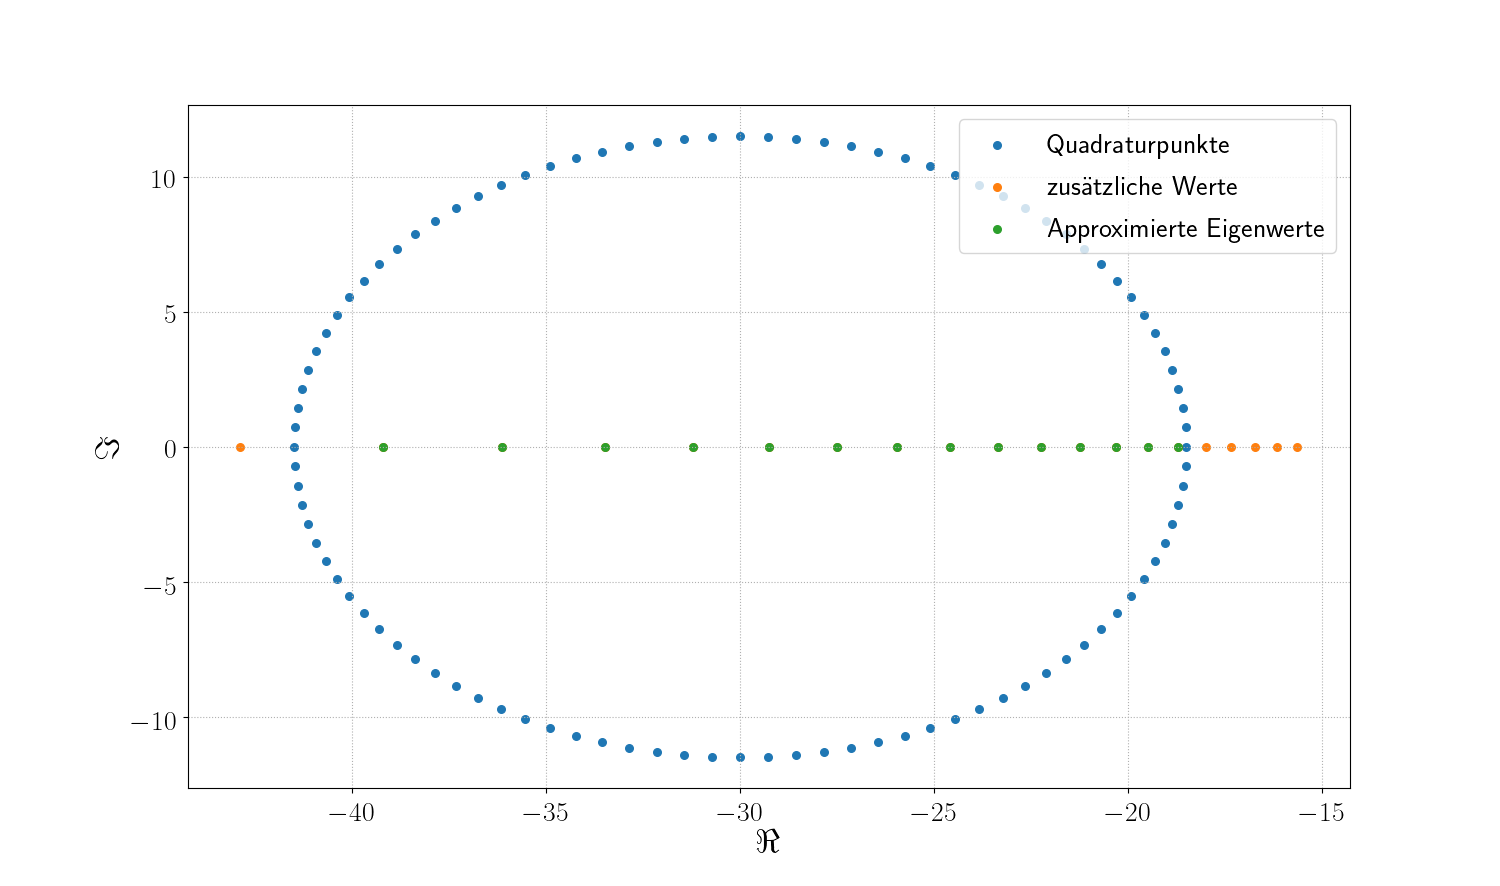
\includegraphics[width = \linewidth]{Plots/eigenwerte_complex_plot.png}
  \caption{Approximierte Eigenwerte vs. zusätzliche Werte}
  \label{fig:plot1}
\end{figure}

\section{Cut-Off}

In Abbildung \ref{fig:plot2} sehen wir den Vergleich der Größenordnungen der eigentlichen Singulärwerte mit den zusätzlichen Singulärwerten.
Nachdem hier ein deutlicher Abfall zu erkennen ist, ist es nicht schwer, die zusätzlichen Werte auszusortieren.

\begin{figure}[H]
  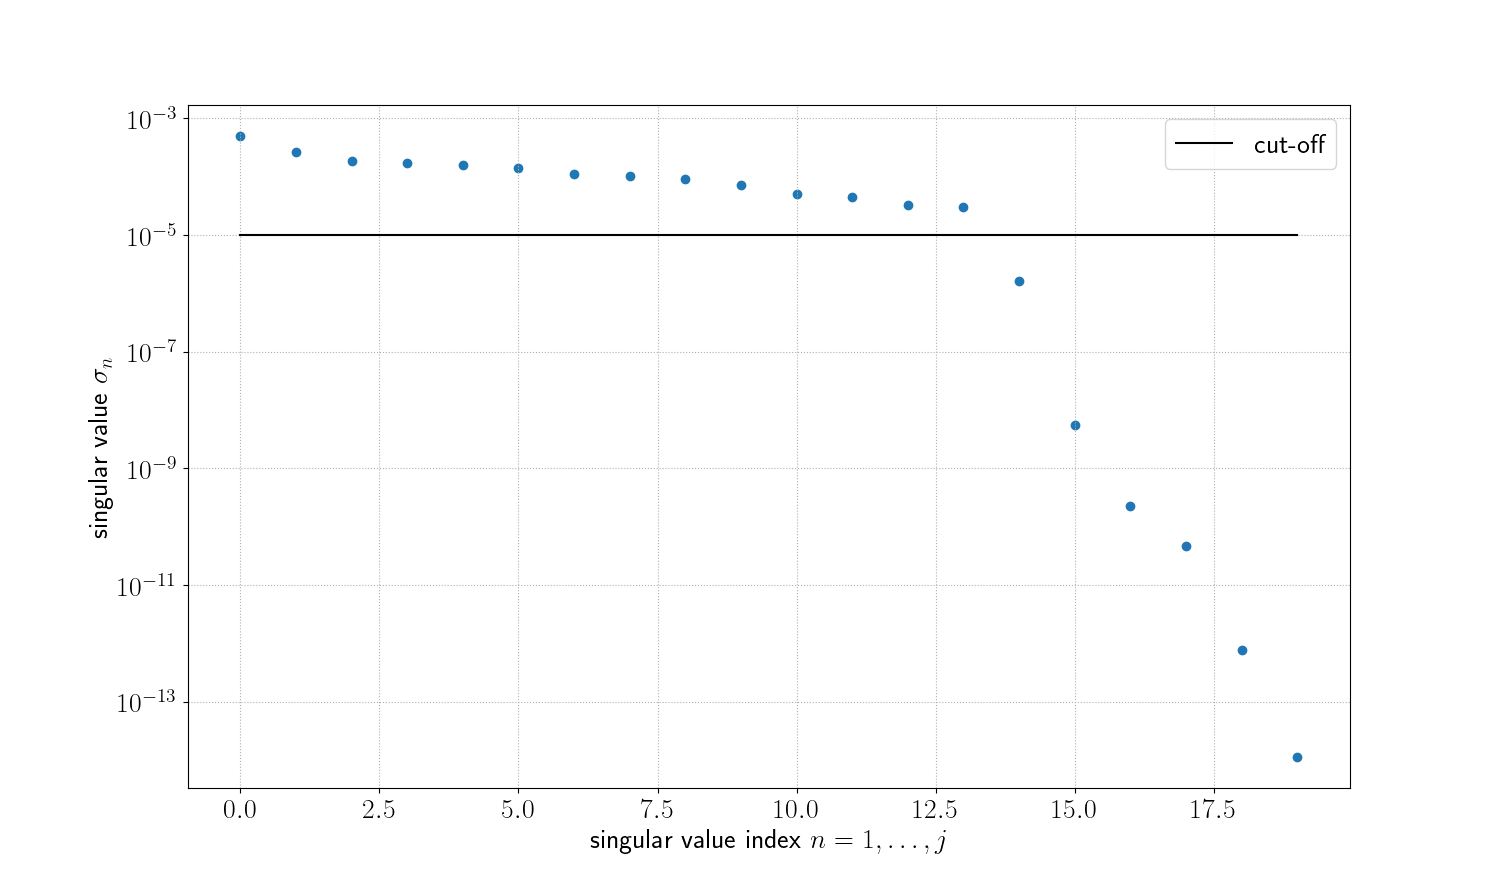
\includegraphics[width = \linewidth]{Plots/singulaerwerte_plot.png}
  \caption{Echte vs. zusätzliche Singulärwerte}
  \label{fig:plot2}
\end{figure}

Eine Heuristik zur Überprüfung der Qualität eines approximierten Eigenwerts $\lambda$ besteht darin, die Konditionszahl der jeweiligen Matrix $A(\lambda)$ zu betrachten.
Da wir gegen eine singuläre Matrix konvergieren sollten, würden wir erwarten, dass die Konditionszahl gegen unendlich geht.
In der Tat ist das Fall und man erkennt in Abbildung \ref{fig:plot3} sogar einen deutlichen Unterschied zwischen den echten und zusätzlichen Eigenwerten.

\begin{figure}[H]
  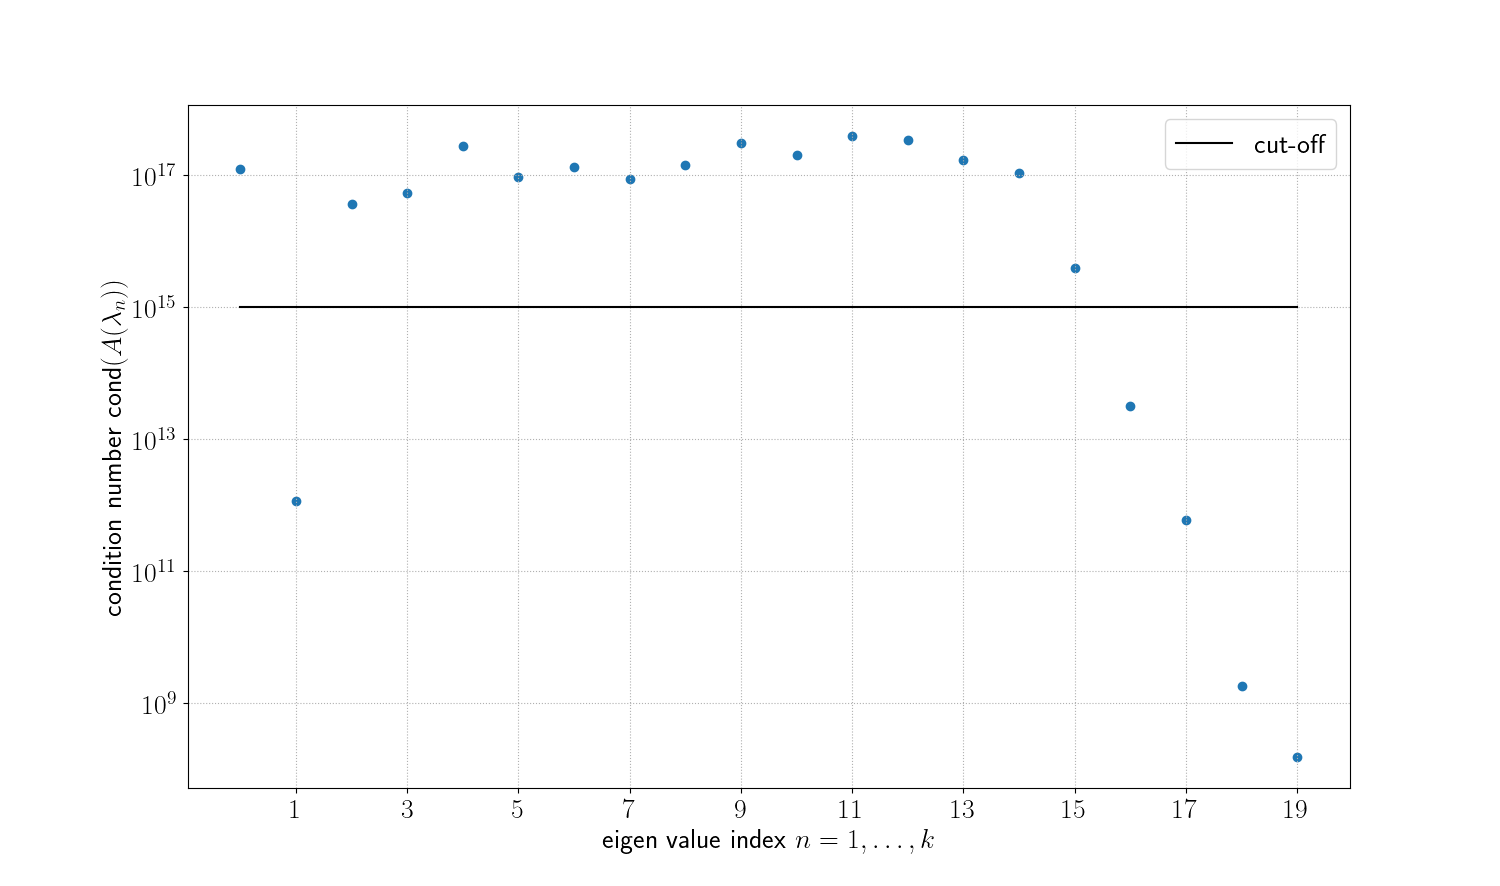
\includegraphics[width = \linewidth]{Plots/conditionnumber.png}
  \caption{Konditionszahlen von $A(\lambda_n)$}
  \label{fig:plot3}
\end{figure}

\section{Pitfalls}

Schlussendlich wollen wir noch Situationen aufzeigen, an denen der Algorithmus scheitert.
Die erste Möglichkeit dafür besteht darin, dass die Quadratur zu ungenau ist, und somit die \blockquote{korrekten} Singulärwerte nicht mehr von den zusätzlichen Werten zu unterscheiden sind.
In Abbildung \ref{fig:plot4} sieht man, wie sich die approximierten Singulärwerte bei unterschiedlicher Anzahl von Quadraturknoten verhalten.
Ab $\texttt{m} \geq 20$ Quadraturknoten aufwärts ist bereits ein Sprung zwischen den echten und zusätzlichen Werten zu erkennen, der sich bei steigender Anzahl noch verdeutlicht.

\begin{figure}[H]
  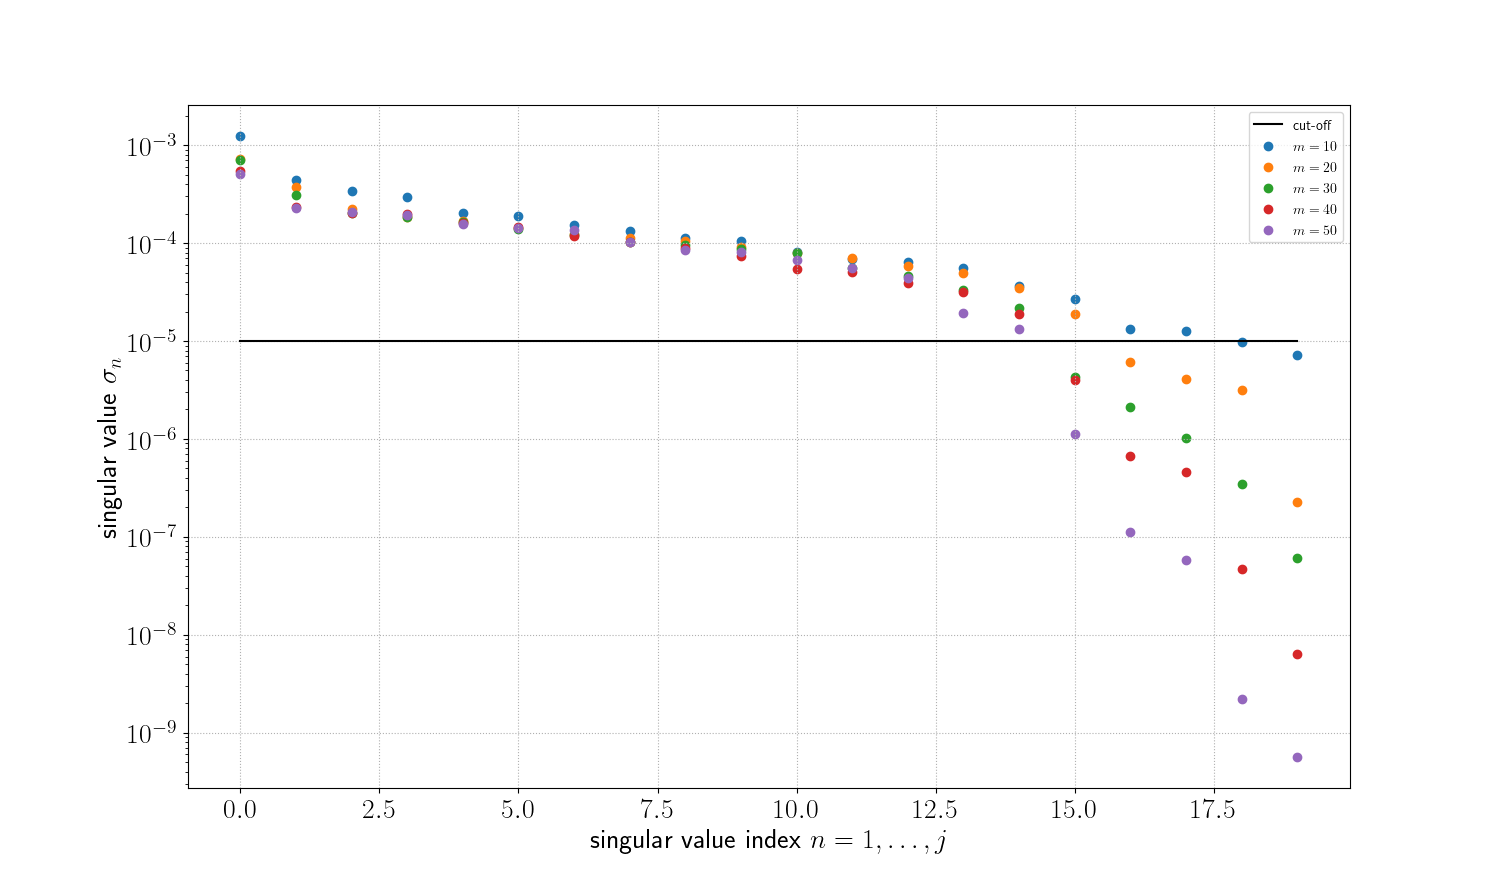
\includegraphics[width = \linewidth]{Plots/singulaerwerte_quadraturknoten.png}
  \caption{Singulärwerte in Abhängigkeit von der Anzahl der Quadraturknoten}
  \label{fig:plot4}
\end{figure}

Das zweite Hauptproblem ist, wenn die Zufallsmatrix zu klein gewählt wird.
Sollte die Zufallsmatrix weniger Spalten haben, als wir Eigenwerte innerhalb unserer Kurve erwarten, könnte man ja noch hoffen, zumindest einen Teil der Eigenwerte korrekt approximieren zu können.
Wie man in Abbildung \ref{fig:plot5} sieht, können wir in der Regel nicht einmal das erwarten.

\begin{figure}[H]
  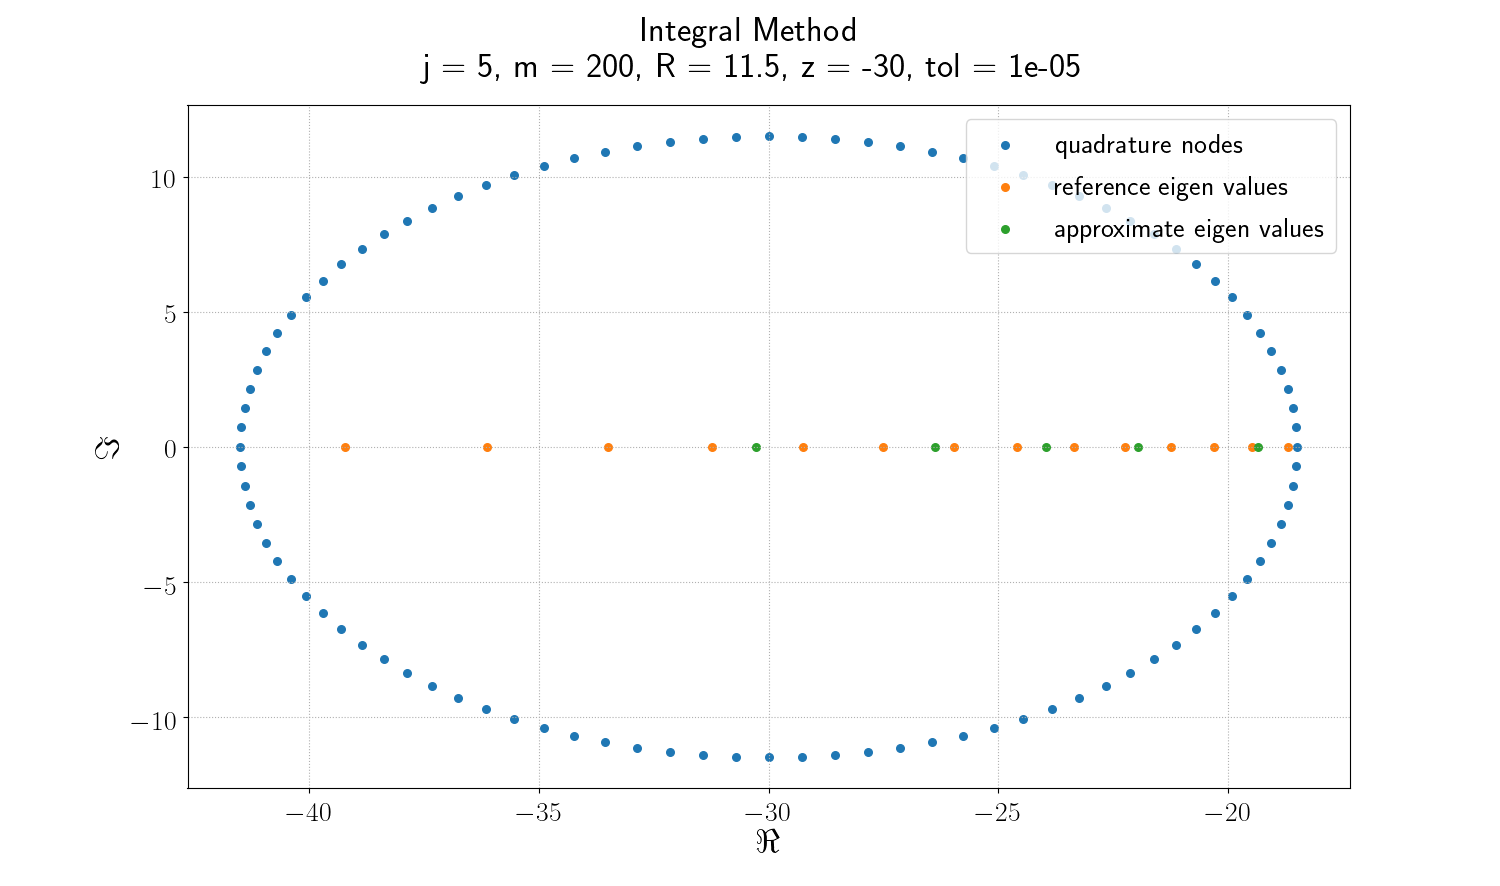
\includegraphics[width = \linewidth]{Plots/zufallsmatrix_zu_klein.png}
  \caption{Zu kleine Zufallsmatrix}
  \label{fig:plot5}
\end{figure}


    \chapter{Fazit}

Die Konturintegral-Methode ist ein Verfahren zur Lösung nichtlinearer Eigenwertprobleme, basierend auf dem \blockquote{Satz von Keldysh}.
Die zentrale Formel, die dem Algorithmus zu Grunde liegt ist

\begin{gather*}
    \frac{1}{2 \pi i}
    \Int[\Gamma]{f(\lambda) A(\lambda)^{-1}}{\lambda}
    =
    \sum_{n=1}^k
        f(\lambda_n)
        \sum_{l=1}^{L_n}
            v_{n, l} w_{n, l}^\ast.
\end{gather*}

Um den Algorithmus durzuführen, müssen wir die Matrizen

\begin{align*}
    A_0
    & :=
    \frac{1}{2 \pi i}
    \Int[\Gamma]{\lambda^0 A(\lambda)^{-1} \hat V}{\lambda}
    =
    V D^0 W^\ast \hat V
    \in
    \C^{N \times j}, \\
    A_1
    & :=
    \frac{1}{2 \pi i}
    \Int[\Gamma]{\lambda^1 A(\lambda)^{-1} \hat V}{\lambda}
    =
    V D^1 W^\ast \hat V
    \in
    \C^{N \times j}
\end{align*}

mit der Quadratur-Formel

\begin{gather*}
    Q(f)
    :=
    \frac{1}{2 \pi i}
    \Int[|\lambda| = R]{f(\lambda)}{\lambda}
    \approx
    Q_m(f)
    :=
    \frac{R}{m}
    \sum_{\nu = 0}^{m-1}
        \omega_m^\nu f(R \omega_m^\nu), \\
    \omega_m
    :=
    \exp \frac{2 \pi i}{m},
    \quad
    R > 0,
    \quad
    m \in \N,
    \quad
    f \in H(\C),
\end{gather*}

approximieren, die reduzierte Singulärwertzerlegung

\begin{align*}
    A_0
    =
    \tilde V \Sigma \tilde W^\ast
\end{align*}

bestimmen und das lineare Eigenwertproblem der Matrix

\begin{align*}
    \tilde V^\ast A_1 \tilde W \Sigma^{-1}
    \sim
    D
    =
    \operatorname{diag}(\lambda_1, \dots, \lambda_k)
\end{align*}

(beispielsweise mit dem QR-Verfahren) lösen.

Die Integralmethode zur Berechnung der Eigenwerte nichtlinearer Eigenwertprobleme ist vergleichsweise neu und Gegenstand aktueller Forschung.
Die Methode hat die Lösung von nichtlinearen Eigenwertproblemen deutlich vereinfacht, dennoch birgt sie auch wesentliche Probleme.
Neben dem relativ hohen Aufwand wird durch die Verwendung von $A_{0, 1}^{(m)}$ die Anzahl der nicht-verschwindenden Singulärwerte deutlich erhöht.
Solange die \blockquote{korrekten} Singulärwerte um Größenordnungen über den zusätzlichen liegen, können letztere einfach aussortiert werden.
Sind die Approximationen von $A_0, A_1$ nicht genau genug, kann es passieren, dass die \blockquote{korrekten} Singulärwerte kaum mehr von den zusätzlichen Singulärwerten zu unterscheiden sind, und der Algorithmus eventuell falsche Resultate liefert.

Dennoch hat die Integralmethode die Lösung von nichtlinearen Eigenwertproblemen massiv vereinfacht.
Sie ermöglicht bei entsprechender Genauigkeit die zuverlässige Berechnung aller Eigenwerte innerhalb einer gewählten Kurve.
Dies ist ein sehr großer Vorteil zu iterativen Verfahren, bei denen typischerweise die Lage der gefundenen Eigenwerte nicht zuverlässig kontrolliert werden kann.

    \chapter{Anhang}

Hier wollen wir den wesentlichen Backend-Code explizit auflisten.
Dieser baut auf den Paketen \texttt{numpy} (als \texttt{np}), und \texttt{linalg} von \texttt{scipy} auf.

\section{Quadraturformeln}

\lstinputlisting
[
    style = fundament,
    firstline = 10,
    lastline = 20
]
{Code/outsource.py}

\section{Konturintegral-Methode}

\lstinputlisting
[
    style = fundament,
    firstline = 24,
    lastline = 111
]
{Code/outsource.py}


    \printbibliography

\end{document}
